%% LyX 1.3 created this file.  For more info, see http://www.lyx.org/.
%% Do not edit unless you really know what you are doing.
\documentclass[english,20pt,dvips]{foils}
\usepackage[T1]{fontenc}
\usepackage[latin1]{inputenc}
\usepackage{pifont}
\usepackage{amsmath}
\usepackage{graphicx}
\usepackage{amssymb}
\IfFileExists{url.sty}{\usepackage{url}}
                      {\newcommand{\url}{\texttt}}

\makeatletter

%%%%%%%%%%%%%%%%%%%%%%%%%%%%%% LyX specific LaTeX commands.
%% Because html converters don't know tabularnewline
\providecommand{\tabularnewline}{\\}

%%%%%%%%%%%%%%%%%%%%%%%%%%%%%% Textclass specific LaTeX commands.
 \newenvironment{lyxcode}
   {\begin{list}{}{
     \setlength{\rightmargin}{\leftmargin}
     \setlength{\listparindent}{0pt}% needed for AMS classes
     \raggedright
     \setlength{\itemsep}{0pt}
     \setlength{\parsep}{0pt}
     \normalfont\ttfamily}%
    \item[]}
   {\end{list}}

%%%%%%%%%%%%%%%%%%%%%%%%%%%%%% User specified LaTeX commands.


\AtBeginDocument{
  \renewcommand{\labelitemi}{\ding{122}}
  \renewcommand{\labelitemii}{\ding{229}}
}

\usepackage{babel}
\makeatother
\begin{document}

\leftheader{Neil Lawrence}


\rightheader{Network Performance Analysis}


\MyLogo{\includegraphics[%
  scale=0.4]{/share/mlhome/neil/tex/inputs/sheffieldlogo.eps}}


\rightfooter{\includegraphics[%
  scale=1.4]{/home/neil/tex/inputs/dcslogo.eps}\quad \thepage{}}


\title{Network Performance Analysis}


\author{Neil Lawrence}


\date{Autumn Term 2004-2005}

\maketitle

\rotatefoilhead[-0.5in]{Lectures and Tutorials}

\begin{description}
\item [Lectures]Mondays 15:10 - 17:00 pm (St Georges LT1) 
\item [Tutorials]Tuesdays 16:10 pm - 17:00 pm (St Georges LT22). First
one Week 3 - Tonatiuh Pena Centeno is your teaching assistant. 
\item [Evaluation]Exam. 
\item [Reading~Week]The reading weeks will be week 11 \& 12.
\end{description}

\rotatefoilhead[-0.5in]{Reading List}

The course is based primarily on \cite{Bertsekas:data92}. The relevant
parts of the book are as follows. 

\begin{description}
\item [Chapter~1]For background reading and review. 
\item [Chapter~3]Section 3.1 -- 3.5 For queueing models. 
\item [Chapter~4]In less detail: Section 4.1 -- 4.4, Section 4.5.2, 4.5.3. 
\end{description}
For additional background reading you may wish to consult some of
the books listed below, \cite{Tanenbaum:computer96} is the standard
text for Introductory courses, but has little coverage on queueing
theory. \cite{Chan:performance00} is an alternative text for details
on queues.

There is additional material on-line at the course web-site: \url{http://www.dcs.shef.ac.uk/~neil/campus_only/com6131/}.


\rotatefoilhead[-0.5in]{Introduction and Background}


\rotatefoilhead[-0.5in]{Introduction}

Welcome to Network Performance Analysis, 20 lectures and lab sessions
on queueing theory and network simulation. In the first lectures we
will try and place the theory that is to follow in some context. 

Queueing theory dates back to the beginning of the 20th Century and
the pioneering work of \textbf{Agner Krarup Erlang} (1878-1929) a
Danish Telecoms Engineer who published the first paper on queueing
theory \cite{Erlang:theory09}. 

In these first two lectures we will introduce the background for the
material which follows: the development of worldwide communication
networks. For further reading please check \url{http://www.wikipedia.org}
and \url{http://www.computerhistory.org}.


\rotatefoilhead[-0.5in]{Early Milestones}

Perhaps the first major development in telecommunications was \emph{the
telegraph}. \textbf{Samuel F. B. Morse} developed ideas for the electrical
telegraph which exploited the relationship between magnetism and electricity.
His first working system sent a short message from Baltimore to Washington
D.C. (two cities that are conveniently close together!). It was sent
on May 24th, 1844: `What hath God wrought?'. Ten years later 23,000
miles of wire across the United States. 

At the time, a key limitation of the telegraph was that it only provided
one channel per wire for communication. Work in using a single wire
for multiple channels (multiplexing) indirectly led to the invention
of \emph{the telephone} which was patented by \textbf{Alexander Graham
Bell} (1847-1922) in March 7th, 1876.

The development of a \emph{wireless telegraphy} system by the Italian
born engineer \textbf{Guglielmo Marconi} (1874-1937), patented in
July 1897, led to the foundation of the Wireless Telegraph \& Signal
Company. By December 1901 short wave transmission across the Atlantic
between England and Canada (over 2,100 miles). 


\rotatefoilhead[-0.5in]{Automated Telephone Networks}

Initially, telephone call routing was achieved manually. Operators
at the exchange used patch boards to make physical connections between
the callers. The invention, by \textbf{Almon Strowger} (1839-1902),
of the \emph{automatic telephone exchange} (through the Strowger switch)
in 1891 brought about the need for a theoretical study of the operation
of telephone exchanges. 

The network of interconnected phone lines is now known as a \emph{circuit
switching network}. It is a network of lines which can be switched
between two subscribers to form a connection. 

Erlang's contribution was to provide theoretical studies of these
networks which allowed telephone exchanges to be designed to meet
demand.


\rotatefoilhead[-0.5in]{Information Theory}

As 'phone networks developed the need for underlying theory grew.
Networks transmit `information' but to discuss concepts such as channel
capacity with out a formal definition for information is meaningless.
\textbf{Claude E. Shannon} (1916-2001) wrote a seminal paper \emph{A
Mathematical Theory of Communication} \cite{Shannon:info48} which
founded the field of information theory and revolutionized the way
we look at telecommunication. This work enabled us to discuss concepts
such as the capacity of a channel with a well founded underlying mathematical
theory. We will not cover the ideas from this course here, but some
students will learn more about this in the module COM6862: \emph{Applications
of Coding, Information and Learning Theories}.


\rotatefoilhead[-0.5in]{Computer Networks}

Circuit switched networks were designed for telephone communication
between two correspondents. These were the first worldwide communication
networks. However, by the early 1960s the need for a new type of communication
network was arising. In circuit switching networks, a permanently
open line connects the correspondents. A fixed bandwidth is available
to them for communication. If they do not use this bandwidth it cannot
be made available to other network users. In \emph{packet switching
networks} or store and forward switching networks the bandwidth is
not reserved in this way: it is distributed across the network user
base. The information a user sends (whether it be voice like in a
phone conversation and VoIP%
\footnote{Voice over IP, the protocol for having phone conversations over the
internet.%
} or a file using FTP%
\footnote{FTP is the file transfer protocol, a much older protocol which dates
back to the formation of the ARPANET.%
}) is split into packets which are routed across the network to the
desired destination. If a required communication line is in use the
packet is stored in a queue until the line becomes available (thus
the name store and forward switching). The ideas behind packet switching
networks were developed independently by \textbf{Paul Baran} (1926-)
at the RAND corporation in the U.S. and \textbf{Donald Davies} (1924-2000)
of the National Physical Laboratory in the U.K.. \textbf{Leonard Kleinrock's}
(1934-) 1962 thesis (later published as a book \cite{Kleinrock:communication64})
provided a mathematical theory that underpinned these networks.




\rotatefoilhead[-0.5in]{ARPANET}

The Advanced Research Projects Agency (ARPA) funded a network that
actually implemented these ideas. In 1969 the ARPA network connected
four nodes at the University of California, Los Angeles (UCSB); the
Stanford Research Institute; the University of California, Santa Barbara
(UCSB) and the University of Utah. By 1975 (see Figure~\ref{cap:arpaNet1975})
the network had expanded to cover most of the major universities (61
nodes) in the U.S. as well as a node at University College London
in the U.K..

%
\begin{figure}[ht]
\begin{center}\includegraphics[%
  scale=0.75]{diagrams/1975_net_map.gif}\end{center}


\caption{The ARPANET in 1975, image courtesy of the Computer History Museum,
\protect\url{http://www.computerhistory.org}. Some abbreviations:
UCB - University of California at Berkeley; UCSD - University of California
at San Diego; UCLA - University of California at Los Angeles; PDP-XX
- the PDP machines were early mini-computers made by DEC with a price
tag of around \$20,000. The machines starting with 360 and 370 are
IBM mainframe machines. Note the transatlantic link to London and
the link over the Pacific to Hawaii. There are 61 nodes in total on
this network.\label{cap:arpaNet1975}}
\end{figure}
ARPANET was the first network for computer communications, it was
restricted to non-commercial use and funded by ARPA and NSF until
1990. With the increase in communication, protocols became far more
important. Just as spellings of European languages became standardised
after the introduction of the the printing press communication protocols
also became more prevalent. Telnet and file transfer protocols (FTP)
were developed in 1971, but perhaps the most important protocol developed
at that time was the transmission control protocol (TCP) developed
in the mid-seventies by \textbf{Vinton G. Cerf} (1943-) and \textbf{Robert
E. Kahn} (1938-) \cite{Cerf:packet74}. These protocols allow interconnection
between networks thereby enabling the formation of the internet.


\rotatefoilhead[-0.5in]{The Internet }

By 1977 Cerf and Kahn were able to send messages across networks including
the `Packet Radio net', SATNET and the ARPANET. At a similar time
Robert Metcalfe (1946-) was developing Ethernet at Xerox PARC. Ethernet
was inspired by the ALOHA networks at the University of Hawaii. Each
machine in the ALOHA network communicated across the same frequency
radio channel. This meant that if several communications where sent
at the same time `collisions' could occur resulting in garbled messages.
A procedure for detecting and retransmitting the message was required.
For Ethernet networks a cable is the medium of transmission, rather
than a radio frequency. Ethernet was supported by an alliance of companies:
DEC, Intel and Xerox. This led to Ethernet networks superseding other
competing approaches such as token ring, FDDI and ARCNET. The cheap
availability of Ethernet and computers in general contributed to an
explosion in the number of networks associated with the internet.

By 1990 when ARPANET was formally shutdown it had grown to 300,000
hosts and connected countries across the globe, it evolved into the
NFSNet which became the backbone of the internet. In 1991 the internet
was opened to commercial traffic, the commercialisation of the internet
in combination with the invention of the hyper-text markup language
(HTML) and universal resource locaters (URL) by \textbf{Tim Berners-Lee}
(1955-) formed the foundations of the modern internet.


\rotatefoilhead[-0.5in]{Network Performance Analysis}

In this course we will introduce you to the tools for design and analysis
of telecommunications networks. The core tools of this analysis are
probability based: there is an assumption that the traffic in the
system is stochastic. 

The techniques we will cover are applicable beyond the design and
analysis of telecommunication networks. Queues form in a variety of
Information Technology scenarios: compute servers dealing with submitted
jobs and databases handling queries. They also occur in our every
day lives: cashpoints, supermarkets, registration, telephone call
centres \emph{etc}.. The principles we will cover apply in each of
these situations. 


\rotatefoilhead[-0.5in]{Server Design}

As a simple example let's consider a database (perhaps MySQL). We
are constructing it from existing parts. We have two CPU/motherboard
systems and two separate disk systems, their expected characteristics
are shown in Table~\ref{cap:SQLserver}. Which should we match with
which? Are we better off building one faster system and one slower
system? Or should we build two systems that have a similar performance?

%
\begin{table}[ht]
\begin{center}\begin{tabular}{|c|c|c|c|}
\hline 
CPU System&
Expected Service Time/ms&
Disk System&
Expected Service Time/ms\tabularnewline
\hline
\hline 
A&
423&
1&
215\tabularnewline
\hline 
B&
210&
2&
390\tabularnewline
\hline
\end{tabular}%~\vspace{4cm}
\end{center}


\caption{Average times for a fictional database server for three different
cases.\label{cap:SQLserver}}
\end{table}



\rotatefoilhead[-0.5in]{Practical Considerations}

For the moment, let's focus on, for example, network design. Broadly
speaking we need to focus on two interrelated areas in our analysis:

\begin{enumerate}
\item \textbf{Design Issues}: when building or buying a router how much
memory should we allow for? How much bandwidth do we need between
routers? How much processing power should the router have so that
it may exploit that bandwidth effectively?
\item \textbf{Quality Issues}: what will be the average delay for end users
given our network design? What is the worst case delay? How likely
is the system to drop packets?
\end{enumerate}
These are important because resources are finite, there are limitations
on the available bandwidth, processor speeds and memory. 


\rotatefoilhead[-0.5in]{Terminology}

Before we cover these issues in more detail, let's introduce some
standard terminology. Typically a series of communications between
two users/computers is known as a \emph{session}. The interactions
themselves consist of \emph{messages} each of which may be split into
\emph{packets}. 

One example of a session would be a lecture. The session consists
of a mainly one-way communication between me, the server, and you
multiple clients. In this case most of the information transfer is
one-way with me sending a series of messages, each involving a different
subject: my identity, the history of communication, this course's
subject matter \emph{etc}. and you acknowledging by your lively reactions.
Each message consists of a series of packets, in this case perhaps
the sentences that I speak. The communication medium is the air between
us. 


\rotatefoilhead[-0.5in]{Session Characteristics}

Depending on the nature of the information communicated between the
client and the server the characteristics of the session can vary
dramatically. An FTP session may involve a few packets from the client
to request a file followed by many packets from the server to send
the file. A VoIP session will involve large numbers of packets between
two users and no obvious client/server relationship. An hypertext
transfer protocol (HTTP) session may involve long periods of inactivity
as the client reads the pages they have downloaded.

Each of the following six criteria/characteristics of a session may
need to be considered in the design of the protocol and the network.

\begin{enumerate}
\item \textbf{Message arrival rate}. We can seek to model the arrivals as:
\emph{Poisson arrivals}, \emph{deterministic arrivals}, \emph{uniform
arrivals} or as coming from a more general class of distributions.
\item \textbf{Session holding time}: The length of a session.
\item \textbf{Expected message length} and \textbf{length distribution},
message lengths can be modeled as \emph{exponential distributions},
\emph{uniform length}.
\item \textbf{Allowable delay} - acceptable expected delays vary. The acceptable
delay is low for VoIP and quite high for FTP. 
\item \textbf{Reliability} - FTP \emph{must} be error free but VoIP can
have some bit errors or packet loss without major consequences.
\item \textbf{Message and packet ordering} - Some sessions will require
that the packets arrive in the order they are sent: for example database
requests.
\end{enumerate}
In this course we will be particularly interested in the first five
of these characteristics. 


\rotatefoilhead[-0.5in]{Network Types}

In our review of the history of communication networks, we have already
met two distinct kinds of network. 

\begin{description}
\item [Circuit~Switching:]used for telephone routing. Guarantees an open
`channel' between two peers. 
\item [Packet~Switching]or Store and Forward Switching: used for data.
May operate via 

\begin{description}
\item [Dynamic~Routing]Each packet of the message moves through the network
independently. 
\item [Virtual~Circuit~Routing]A fixed path through the network is provided
for the entire message. 
\end{description}
\end{description}

\rotatefoilhead[-0.5in]{Characteristics of the Systems}

The character of the two approaches are quite different.


\rotatefoilhead[-0.5in]{Circuit~Switching}

Circuit switching can be wasteful in terms of bandwidth. The communicating
nodes may not be using all the available bandwidth reserved for them
all of the time. However, once connection is established, a guaranteed
channel is provided with a known communication delay associated with
it. 

In a circuit switching network, the sum of rates for all sessions
using a link cannot exceed the total capacity of the link. New sessions
must be rejected when the link capacity is reached. The approach is
used for telephone networks where the session rate, $r_{s}$, is the
same for each session. Switching would be more complex for data networks
and the nature of transmission would also mean that the links are
inefficiently used. 


\rotatefoilhead[-0.5in]{Packet Switching}

Packet switching makes efficient use of bandwidth because, whilst
communication between two nodes may be idle for a period of time,
packets from another communication may be sent along the same line.
However because it is unknown \emph{a priori} how much bandwidth will
be available it is difficult to guarantee a maximum delay. 


\rotatefoilhead[-0.5in]{Illustrative Example}

Alice and Bob both have telephone lines. Alice decides to call Bob
using the phone line. Here the make use of a circuit switching network
provided by their telephone supplier (Figure~\ref{cap:circuitSwitch}).
The session dominates both phone lines preventing use by other `clients'.

%
\begin{figure}[ht]
\begin{center}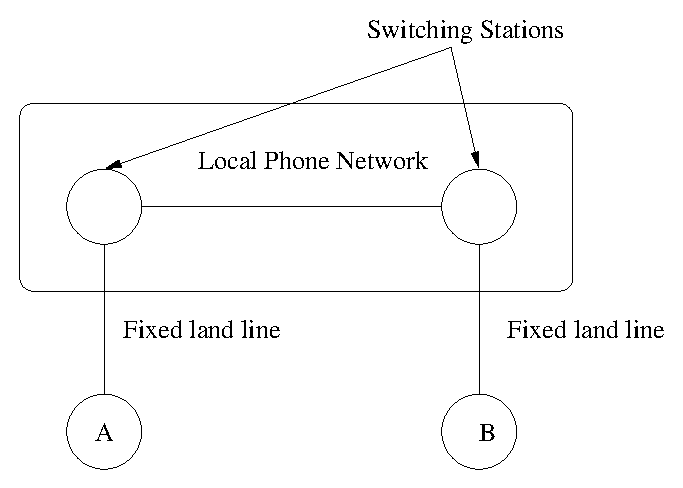
\includegraphics[%
  width=0.70\textwidth]{diagrams/aliceBobCircuit.eps}%~\vspace{4cm}
\end{center}


\caption{A simple circuit switching network connecting Alice and Bob.\label{cap:circuitSwitch}}
\end{figure}


Alternatively Alice and Bob use MSN messenger to communicate (either
via voice or typing), and Bob's friend Carol shares his fixed land
line connection to access David's web server (Figure~\ref{cap:packetSwitch}).

%
\begin{figure}[ht]
\begin{center}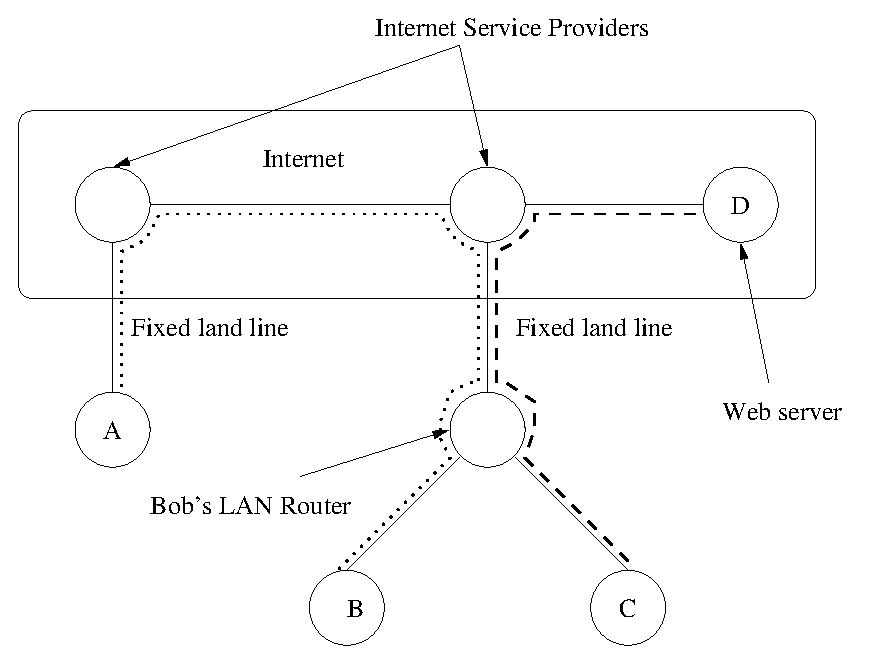
\includegraphics[%
  width=0.70\textwidth]{diagrams/aliceBobPacket.eps}%~\vspace{4cm}
\end{center}


\caption{A simple packet switching network connecting Alice, Bob, Carol and
David.\label{cap:packetSwitch}}
\end{figure}


Now the fixed land line is managed by some form of router in the local
area network in Bob's house. The advantage is that Bob and Carol may
both use the land line for communication the disadvantage is that
if the land line becomes congested \emph{e.g.} as a result of Carol
downloading a large file from David's web server, Bob will notice
a variable delay (delays also occur with circuit switching but they
are known as transmission delays and should be of fixed length) in
his communication with Alice due to queueing occurring at his Internet
Service Provider and in his LAN's router. This can be particularly
irritating for voice conversation, as anyone who has used MSN messenger
for voice communication will attest. 


\rotatefoilhead[-0.5in]{The Layered Model}

We now review the layered model for TCP/IP networks, you are referred
to Tanenbaum (4th Edition pg. 41) for more details.

%
\begin{figure}[ht]
\begin{center}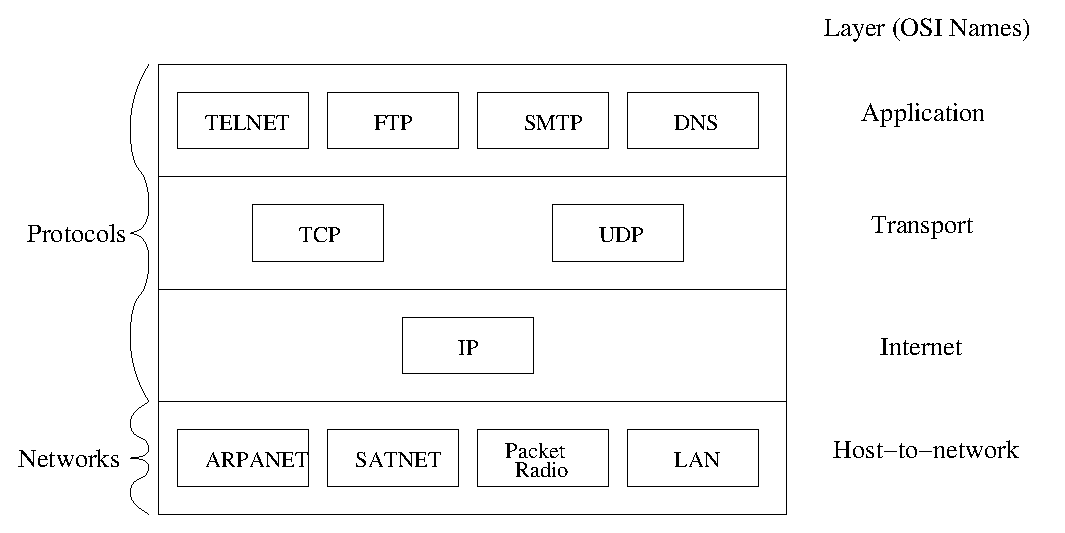
\includegraphics[%
  width=0.70\textwidth]{diagrams/layeredModel.eps}%~\vspace{6cm}
\end{center}


\caption{A schematic of the Layered model for TCP/IP networks.}
\end{figure}


The traditional OSI Reference model contains seven layers which reflect
in a network how communication occurs at different layers using different
protocols. By way of reviewing the TCP model we introduce a layered
representation of the TCP/IP model which underlies the internet. As
we mentioned above TCP/IP was introduced in 1974 as a standard which
interconnects between networks. This is achieved through the Internet
Protocol. The TCP/IP reference model is much more compact and will
serve as a useful reminder.

\begin{description}
\item [Application~Layer]This layer represents the interface to the user
and consists of applications which are commonly used by users. As
well as the examples in the diagram packetised voice communications,
electronic news, HTTP and its secure variants etc.
\item [The~Transport~Layer]The layer above the internet layer is known
as the transport layer and contains two protocols. The Transmission
Control Protocol (TCP) allows applications to communicate in a lossless
manner, \emph{i.e.} any packets which are dropped are retransmitted.
It also implements flow control in an effort to prevent network congestion
and reorders arrivals at the destination. The User Datagram Protocol
(UDP) is an unreliable protocol for applications which wish to provide
their own sequencing and flow control (e.g. voice transmission or
video).
\item [The~Internet~Layer]The key to the success of TCP/IP is the Internet
Protocol. Its objective is to allow the interfacing of different networks
by allowing hosts to place packets on any network and enabling them
to travel to any other network. 
\end{description}

\rotatefoilhead[-0.5in]{Communication Media}

Circuit switching networks may share a communication line but this
is done through multiplexing where a fixed proportion of the communication
channel is dedicated to the session. The multiplexing may be time
division multiplexing or frequency division multiplexing. The former
splits the communication channel into time slots and allocates each
to a different session, the latter uses different portions of the
frequency bandwidth for each channel. Both are not 100\% efficient
(time multiplexing requires a small amount of time for switching to
occur, and frequency division multiplexing requires a small `buffer'
band of frequencies between each session. Packet switching networks
dedicate communication bandwidth to each channel as required. In a
simple first in first out system, packets arrive and, if the queue
is empty, they are transmitted. Otherwise they are stored and await
their turn for transmission. Thus there are two delays: a queueing
delay and a transmission delay. The queueing delay is variable, whilst
the transmission delay will be fixed and given by the packet length
multiplied by the transmission rate of the channel.

Radio transmission is a communication medium which dates back to Marconi.
Transmission may occur across several bandwidths. Traditionally radio
broadcast occurs through frequency division multiplexing. Radio communication
involves taking turns to communicate over the channel (half-duplex).
The most basic wireless packet networks (\emph{e.g.} ALOHA) used one
channel to broadcast their packets over. Delays may occur due to collisions.
A collision is when two systems both attempt to communicate on the
same channel at the same time. Both packets are then lost and such
losses need to be detected.

Similar principles occur for \emph{e.g.} thinwire Ethernet, in this
case the communication medium is a coaxial cable. 


\rotatefoilhead[-0.5in]{The Road Ahead}

\begin{description}
\item [Probability~Review]Review of probability theory. 
\item [Simple~Queuing~models]Simple models of queues based on probability
theory. Little's Law, M/M/1 queue, M/M/$\infty$, M/M/m, M/M/m/m and
M/G/1. 
\item [Simulation]Simulation of queueing systems.
\end{description}

\rotatefoilhead[-0.5in]{Probability Review}

We will now review the basic concepts of probability theory, probability
theory will provide the underlying structure upon which we will base
our models. We will make use of a simple graphical definition to describe
what we mean by probability. For the purposes of this discussion,
we are interested in trials which result in two random variables,
$X$ and $Y$, each of which has an `outcome' denoted by $x$ or $y$.
We summarise the notation and terminology for these distributions
in Table~\ref{cap:basicProbabilityDistributions}.

\begin{center}%
\begin{table}[ht]
\begin{center}\begin{tabular}{|c|c|c|}
\hline 
Terminology&
Notation&
Description\tabularnewline
\hline
\hline 
Joint Probability&
$P\left(X=x,Y=y\right)$&
`The probability that $X=x$ and $Y=y$'\tabularnewline
\hline 
Marginal Probability&
$P\left(X=x\right)$&
`The probability that $X=x$ regardless of $Y$'\tabularnewline
\hline 
Conditional Probability&
$P\left(X=x|Y=y\right)$&
`The probability that $X=x$ given that $Y=y$'\tabularnewline
\hline
\end{tabular}%~\vspace{4cm}
\end{center}


\caption{The different basic probability distributions.\label{cap:basicProbabilityDistributions}}
\end{table}
\end{center}


\rotatefoilhead[-0.5in]{A Graphical Definition of Probability}

A solid understanding of the fundamentals of probability will be one
of the keys to understanding the material in course. We will therefore
quickly review what each of these distributions means with a simple
graphical demonstration. In Figure~\ref{cap:aJointDistribution}
we summarise the outcomes of a series of $N$ trials in a two dimensional
graph.

%
\begin{figure}[ht]
\begin{center}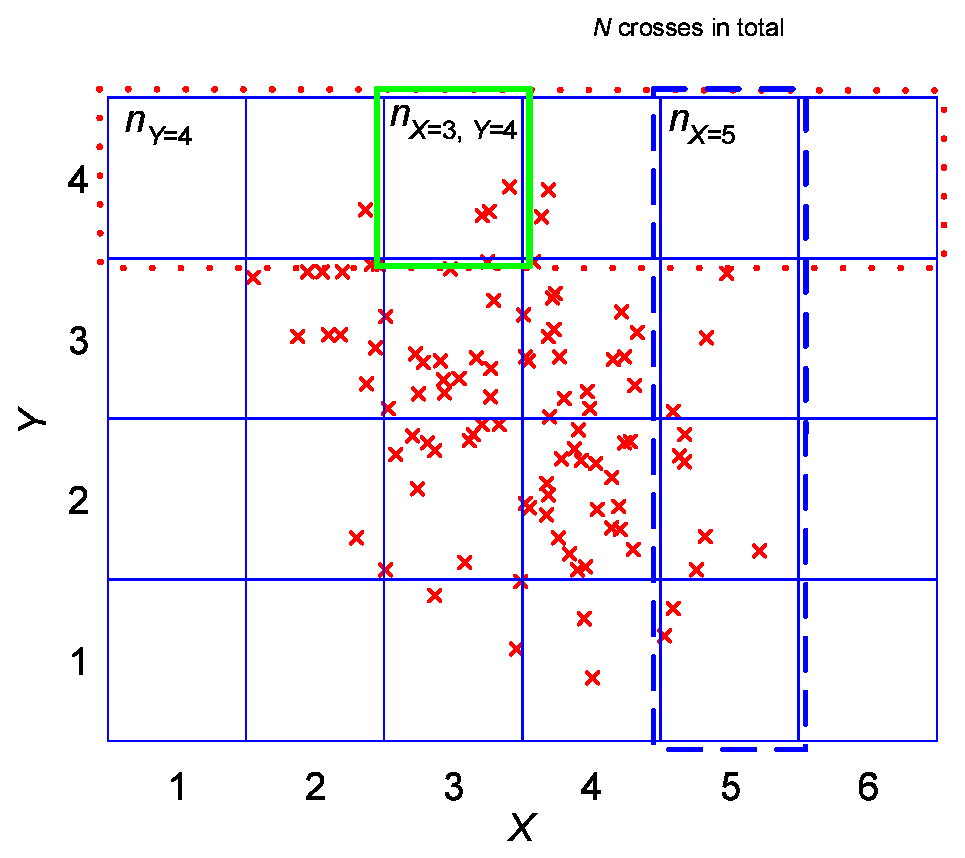
\includegraphics[%
  width=0.80\textwidth]{diagrams/probDiagram.eps}\end{center}


\caption{Representation of joint and conditional probabilities.\label{cap:aJointDistribution}
In this figure the crosses are the outcomes of the trials. They live
in a discrete space of boxes given by the grid. The two events, $X$
and $Y$ are shown across the two axes of the plot.There six possible
outcomes for event $X$, $X=1\dots6$, and five possible outcomes
for event $Y$, $Y=1\dots5$. The small $n$s in the top left hand
corner of each thick lined box denote how many crosses fall inside
that box.}
\end{figure}


For Figure~\ref{cap:aJointDistribution} the outcome of a trial is
plotted on a two dimensional graph. We have drawn three further boxes
on the graph (solid, dotted and dashed lines), each box is defined
by the outcomes it covers. We have denoted the number of events in
each box with a small $n$. Probabilities are defined in the limit
as we take the number of trials $N$ to infinity.

%
\begin{table}[ht]
\begin{center}\begin{tabular}{|c|c|}
\hline 
Terminology&
Definition\tabularnewline
\hline
\hline 
Joint Probability&
$\lim_{N\rightarrow\infty}\frac{n_{X=3,Y=4}}{N}=P\left(X=3,Y=4\right)$\tabularnewline
\hline 
Marginal Probability&
$\lim_{N\rightarrow\infty}\frac{n_{X=5}}{N}=P\left(X=5\right)$\tabularnewline
\hline 
Conditional Probability&
$\lim_{N\rightarrow\infty}\frac{n_{X=3,Y=4}}{n_{Y=4}}=P\left(X=3|Y=4\right)$\tabularnewline
\hline
\end{tabular}%~\vspace{5cm}
\end{center}


\caption{Definition of probability distributions from Table~\ref{cap:basicProbabilityDistributions}
in terms of the system depicted in Figure~\ref{cap:aJointDistribution}.}
\end{table}



\rotatefoilhead[-0.5in]{Notational Details}

Strictly speaking, when we write probability distributions we should
write them out in full (\emph{e.g.} for the joint distribution, $P\left(X=x,Y=y\right)$).
However, in practice, we often use a shorthand notation: $P\left(x,y\right)$.
This is convenient, but it can lead to confusion. It looks very much
like we might write a multivariate function, \emph{e.g.} $f\left(x,y\right)=\frac{x}{y}$.
For a multivariate function though, $f\left(x,y\right)\neq f\left(y,x\right)$
in general. However, for our probability shorthand $P\left(x,y\right)=P\left(y,x\right)$
because $P\left(X=x,Y=y\right)=P\left(Y=y,X=x\right)$.

We have denoted the probability distribution with a capital $P$.
In \emph{these notes} we will use capital $P$s consistently to denote
discrete distributions. Later when we come on to continuous probability
density functions, we will turn to small letters.


\rotatefoilhead[-0.5in]{Probability Rules}

From the simple definitions we've given above we can derive some straightforward
rules associated with manipulating probability distributions. 


\rotatefoilhead[-0.5in]{Normalisation}

The first point to note is that probability distributions are normalised,
the sum over the distribution across each of its possible value is
1. This is clear from the fact that $\sum_{x}n_{X=x}=N$, which gives
\[
\sum_{x}P\left(x\right)=\lim_{N\rightarrow\infty}\frac{\sum_{x}n_{X=x}}{N}=\lim_{N\rightarrow\infty}\frac{N}{N}=1.\]
A similar result can be derived for the marginal and conditional distributions.


\rotatefoilhead[-0.5in]{The Sum Rule }

The sum rule describes how we can obtain a marginal distribution from
the joint distribution. It leads to the terminology marginal distribution
because one of the variables in the joint distribution is marginalised,
\emph{i.e.} it is removed from the distribution (you can think of
it being written in the margin). The marginal probability $P\left(y\right)$
is given by $\lim_{N\rightarrow\infty}\frac{n_{Y=y}}{N}$ and the
joint distribution $P\left(x,y\right)$ is given by $\lim_{N\rightarrow\infty}\frac{n_{X=x,Y=y}}{N}$.
Now we note (using Figure~\ref{cap:aJointDistribution}) that $n_{Y=y}=\sum_{x}n_{X=x,Y=y}$,
where the sum is over all possible values of $X$. We therefore find
that\[
\lim_{N\rightarrow\infty}\frac{n_{Y=y}}{N}=\lim_{N\rightarrow\infty}\sum_{x}\frac{n_{X=x,Y=y}}{N},\]
or in other words\[
P\left(y\right)=\sum_{x}P\left(x,y\right).\]
This is known as the sum rule of probability. 


\rotatefoilhead[-0.5in]{The Product Rule}

The product rule describes how we obtain a joint distribution from
a conditional distribution and a marginal. Recall that the conditional
distribution $P\left(x|y\right)$ is given by $\lim_{N\rightarrow\infty}\frac{n_{X=x,Y=y}}{n_{Y=y}}$.
This can be related to the joint distribution over $x$ and $y$ and
the marginal distribution over $x$ using the fact that $P\left(x,y\right)$
is given by \[
\lim_{N\rightarrow\infty}\frac{n_{X=x,Y=y}}{N}=\lim_{N\rightarrow\infty}\frac{n_{X=x,Y=y}}{n_{Y=y}}\frac{n_{Y=y}}{N}\]
or in other words\[
P\left(x,y\right)=P\left(x|y\right)P\left(y\right).\]
This is known as the product rule of probability.


\rotatefoilhead[-0.5in]{Bayes' Rule}

Less relevant to our work on queueing theory, but worth pointing out
since we've come so far is Bayes' Rule or Bayes' Theorem. Since the
joint distribution is commutative in its arguments we have, from the
product rule,\[
P\left(x,y\right)=P\left(y,x\right)=P\left(y|x\right)P\left(x\right),\]
 it naturally follows that we can write\[
P\left(x|y\right)P\left(y\right)=P\left(y|x\right)P\left(x\right)\]
which leads to Bayes' Rule, which relates the two conditional probabilities
associated with the variables:\[
P\left(x|y\right)=\frac{P\left(y|x\right)P\left(x\right)}{P\left(y\right)}.\]



\rotatefoilhead[-0.5in]{Expectations\label{sec:expectations}}

A probabilistic model of a system may summarise our beliefs about
the system, but to develop further understandings of the model often
want to summarise the model by its expectations.

The expected value of a function, $f\left(x\right)$, under a probability
distribution $P\left(x\right)$ is \[
\left\langle f\left(x\right)\right\rangle _{P\left(x\right)}=\sum_{x}P\left(x\right)f\left(x\right).\]
Here we have introduced a particular notation for the expectation,
you will also see expectations written in the form $E\left\{ f\left(x\right)\right\} $. 


\rotatefoilhead[-0.5in]{Example}

Suppose that $X$ can be $0,\,1,$ or $2$ and $f\left(x\right)=x^{2}$.
We define the distribution over $x$ in Table~\ref{cap:simpleXDistribution}.

%
\begin{table}[ht]
\begin{center}\begin{tabular}{|c|c|c|c|}
\hline 
$x$&
0&
1&
2\tabularnewline
\hline
\hline 
$P\left(x\right)$&
0.2&
0.5&
0.3\tabularnewline
\hline 
$f\left(x\right)=x^{2}$&
0&
1&
4\tabularnewline
\hline
\end{tabular}%~\vspace{4cm}
\end{center}


\caption{Distribution over $x$ and associated values of $f\left(x\right)$.\label{cap:simpleXDistribution}}
\end{table}
 From the definition of an expectation we gave we can compute \[
\left\langle f\left(x\right)\right\rangle =\left\langle x^{2}\right\rangle =0\times0.2+1\times0.5+4\times0.3=1.7,\]
where we have dropped the subscript $P\left(x\right)$, as we consider
it clear from the context what the expectation is considered to be
over. We can also see that the expectation of $x$ under this distribution
is\[
\left\langle f\left(x\right)\right\rangle =\left\langle x\right\rangle =0\times0.2+1\times0.5+2\times0.3=1.1.\]
The expectation of $x$ under a distribution is known as the first
moment of the distribution or its \emph{mean}. The mean can be thought
of as the `centre of probability mass' of the distribution. The expectation
of $x^{2}$ is known as the second moment, it is normally used in
combination with the mean to obtain the variance. 


\rotatefoilhead[-0.5in]{Variance}

The variance of the distribution is given by the difference between
the second moment and the square of the mean. It is often denoted
by $\sigma^{2}$.\[
\sigma^{2}=\left\langle x^{2}\right\rangle -\left\langle x\right\rangle ^{2}.\]
It is always positive and it expresses the degree of variation around
the mean value. Its square root is known as the standard deviation\[
\sigma=\sqrt{\left\langle x^{2}\right\rangle -\left\langle x\right\rangle ^{2}},\]
for our example above the variance is given by\[
1.7-\left(1.1\right)^{2}=0.49,\]
the standard deviation is therefore\[
\sqrt{1.7-\left(1.1\right)^{2}}=0.7.\]



\rotatefoilhead[-0.5in]{Distributions as Functions\label{sec:distributionAsFunction}}

In the above example we defined a probability distribution by a simple
table, making sure that the values summed to 1. A more compact way
to represent a distribution is in terms of a function. As an example
of this we will consider the Poisson distribution. 


\rotatefoilhead[-0.5in]{The Poisson Distribution}

The Poisson distribution was first published by \textbf{Sim\'{e}on
Denis Poisson} (1781-1840) in 1837. It is defined over the space of
all non-negative integers. Since this set is countably infinite in
size it is impossible to write all the numbers down that would define
the distribution. The Poisson distribution is therefore defined as\begin{equation}
P\left(k|\mu\right)=\frac{\mu^{k}}{k!}\exp\left(-\mu\right).\label{eq:poissonDist}\end{equation}
where $k$ is any integer from $0$ to $\infty$, and $\mu$ is a
parameter of the distribution. In these notes we place $\mu$ on the
right of the conditioning bar to indicate that it is a parameter.
Note that in \cite{Bertsekas:data92} a slightly different notation
is used. To work out the probability of a particular value, $k$,
for the a Poisson distribution with a particular parameter, $\mu$,
we simply substitute the parameter and the value $n$ into (\ref{eq:poissonDist}).
For example, with $\mu=2$ we can start filling a table (Table \ref{cap:poissonTable}).%
\begin{table}[ht]
\begin{center}\begin{tabular}{|c|c|c|c|c|}
\hline 
$k$&
0&
1&
2&
$\dots$\tabularnewline
\hline
\hline 
$P\left(x\right)$&
0.135&
0.271&
0.271&
$\dots$\tabularnewline
\hline
\end{tabular}%~\vspace{4cm}
\end{center}


\caption{Some values for the Poisson distribution.\label{cap:poissonTable}}
\end{table}
 


\rotatefoilhead[-0.5in]{Mean and Variance}

We review the mean of a Poisson in the following example. The variance
is an exercise in the first tutorial sheet.

\begin{minipage}[c]{1.0\textwidth}%
~


\rotatefoilhead[-0.5in]{Example: Mean and Variance of Poisson Distribution}

As we mentioned in Section~,\ref{sec:expectations}, the expectations
under a distribution are important for summarising the distributions
characteristics. Expectations of ditributions that take the form of
a function can also be computed. Typically we expect the resulting
expectation to be a function of the distributions parameters.

Let's start with the mean of the Poisson process. \[
\left\langle k\right\rangle _{P\left(k|\mu\right)}=\sum_{k=0}^{\infty}k\frac{\mu^{k}}{k!}e^{-\mu}\]
 To make progress with this we first pull out $\mu e^{-\mu}$ and
the first $k$ in the factorial, $\frac{k}{k!}=\frac{k}{k(k-1)!}=\frac{1}{(k-1)!}$.
We can also remove the first term from the sum because it is multiplied
by $k$ which is zero for the first term.

This leads to\[
\left\langle k\right\rangle =e^{-\mu}\mu\sum_{k=1}^{\infty}\frac{\mu{}^{(k-1)}}{(k-1)!}\]
 Now we make the following substitution: $m=k-1$. \begin{equation}
\left\langle k\right\rangle =e^{-\mu}\mu\sum_{m=0}^{\infty}\frac{\mu{}^{m}}{m!}\label{eq:poissonMean2}\end{equation}
 Now we note that the geometric series $\sum_{m=0}^{\infty}\frac{\mu^{m}}{m!}=e^{\mu}$.
Substituting this result back into (\ref{eq:poissonMean2}) we find
\begin{equation}
\left\langle k\right\rangle =\mu\label{eq:poissonMean3}\end{equation}


The variance of a Poisson is also $\mu$ --- see Tutorial 1. 

%~\vspace{\textheight}
\end{minipage}%



\rotatefoilhead[-0.5in]{Continuous Variables}

So far we have discussed a value for discrtete values of $x$ or $y$.
We now turn to a continuous models. First though we introduce the
probability distribution's sister, the \emph{probability density function}
(PDF). In the discrete case, we defined probability distributions
over a discrete number of states. However, if we wish to model a continuous
value, such as the height of a computer science student, how do we
represent it as a probability distribution? One way would be to `discretise'
the continuous value by splitting it into discrete regions. We effectively
did this in the example in Figure~\ref{cap:aJointDistribution}.
So, for our height example, we could model the probability that your
height was between $1.6\textrm{m}$ and $1.7\textrm{m}$, or alternatively
we could ask what is the probability that you are over $1.8\textrm{m}$
given that you are a computer scientist? However, remodelling for
each of these questions would be rather tedious. It would be more
convenient if we could develop a representation which could answer
\emph{any} question we chose to ask about a computer scientist's height.
This is what a probability density function represents. It does not
represent probabilities directly, but from it they may be derived. 

%
\begin{figure}[ht]
\begin{center}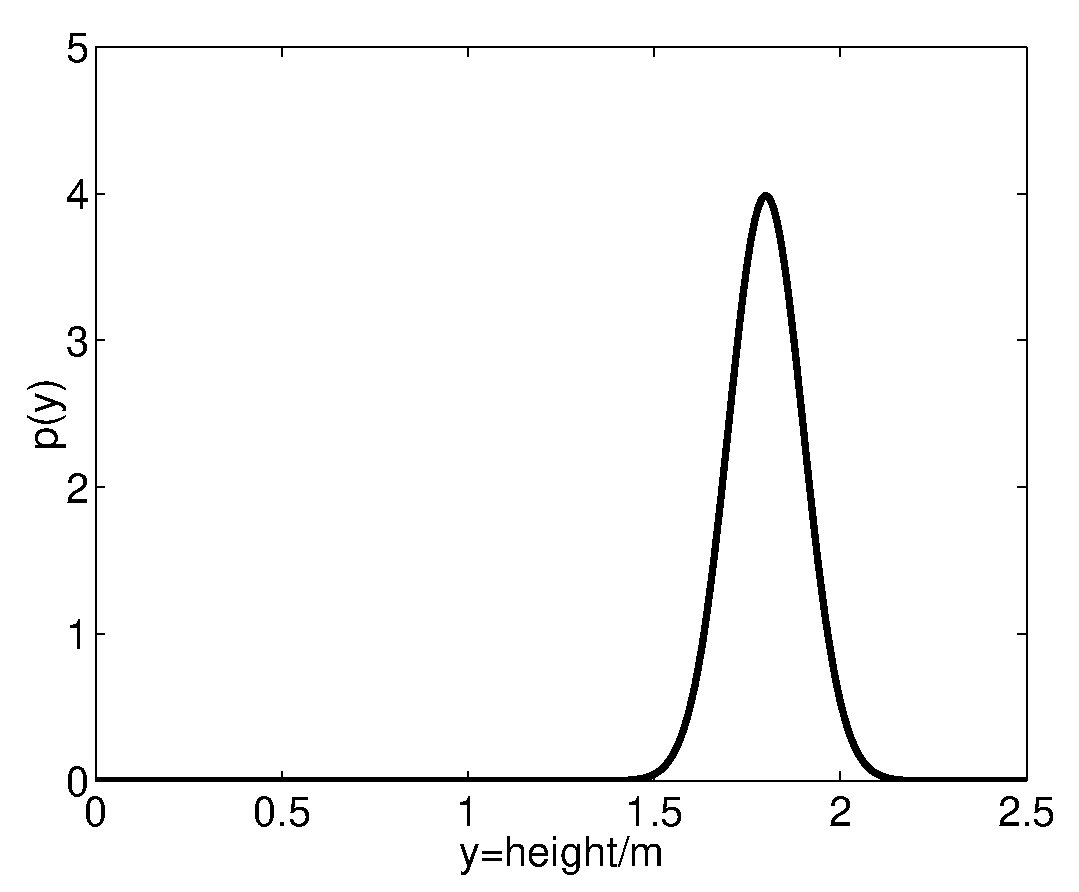
\includegraphics[%
  scale=0.5]{diagrams/pdfOfHeight.eps}\end{center}


\caption{A Gaussian PDF representing heights of computer scientists.\label{cap:heightPDF}}
\end{figure}


We represent a probability density function with a small $p\left(\cdot\right)$
to differentiate it from a probability distribution which we have
denoted with a large $P\left(\cdot\right)$. We define it to be a
positive function whose integral over the region of interest is one%
\footnote{In what follows we shall use the word distribution to refer to both
discrete probabilities and continuous probability density functions.%
}. One example is the Gaussian, shown above to represent a model of
the computer science student's height. We can query the distribution
by integrating over regions of it. If we wish to ask the question
`What is the probability that a computer science student is over $2\textrm{m}$
tall?' The answer, which we denote $P\left(y>2\right)$ is given by
integrating from 2 to $\infty$. Since the total area under the curve
is always one, and the function is always positive. The answer will
always be less than 1 and greater than 0, fulfilling our definition
of probabilities. The answer to the inverse question will be $1-P\left(y>2\right)$.
Note that this implies that the probability of a student being exactly
$2\textrm{m}$ tall is zero. This may seem odd, but is a consequence
of querying the system in the limit as a region tends to zero. 


\rotatefoilhead[-0.5in]{Manipulating PDFs}

The same rules that apply to probability distributions may also be
applied to PDFs. We won't derive this here, but take it as given that\[
p\left(y|x\right)=\frac{p\left(x|y\right)p\left(y\right)}{p\left(x\right)}\]
where $p\left(x,y\right)=p\left(x|y\right)p\left(y\right)$ and for
continuous variables $p\left(x\right)=\int p\left(x,y\right)dy$.
Here the integral is over the region for which our PDF for $y$ is
defined (\emph{e.g.} all real numbers or all positive real numbers).
Additionally we may mix discrete and continuous variables. If, for
example $y$ is discrete and $x$ is continuous then we may write\[
P\left(y|x\right)=\frac{p\left(x|y\right)P\left(y\right)}{p\left(x\right)}.\]
Finally expectations under a PDF are also computed using the integral
instead of the sum so \[
\left\langle f\left(x\right)\right\rangle _{p\left(x\right)}=\int f\left(x\right)p\left(x\right)dx\]
where the integral is over the region for which our PDF for $x$ is
defined.


\rotatefoilhead[-0.5in]{Cummulative Distribution Functions\label{sub:CDFs}}

We've discussed how a PDF doesn't represent probabilities directly,
but it is a mechanism by which questions about the random variable
can be answered. One very common question is: what is the probability
that $x<y$? It can be useful to have a function which stores the
answer to this question for all $y$. This function is known as the
cummulative distribution function (CDF). The CDF is given by the integral
of the PDF across all values of $x$ less than $y$. So if the probability
distribution is valid in the range $-\infty<x<\infty$ the CDF is
given by\[
P\left(x>y\right)=\int_{-\infty}^{y}p\left(x\right)dx,\]
alternatively, if the distribution is defined in the range $0\leq x<\infty$
then the CDF is given by\[
P\left(x>y\right)=\int_{0}^{y}p\left(x\right)dx.\]
To complete the distribution we need the probability that $x\leq y$
(which is the other possibility). This is easy to compute because
we know the distribution must be normalised, $P\left(x\leq y\right)=1-P\left(x>y\right)$.

In Figure~\ref{cap:heightPDF} we give an example of a cummulative
distribution function. We show the CDF associated with the PDF of
the MSc student heights.

%
\begin{figure}[ht]
\begin{center}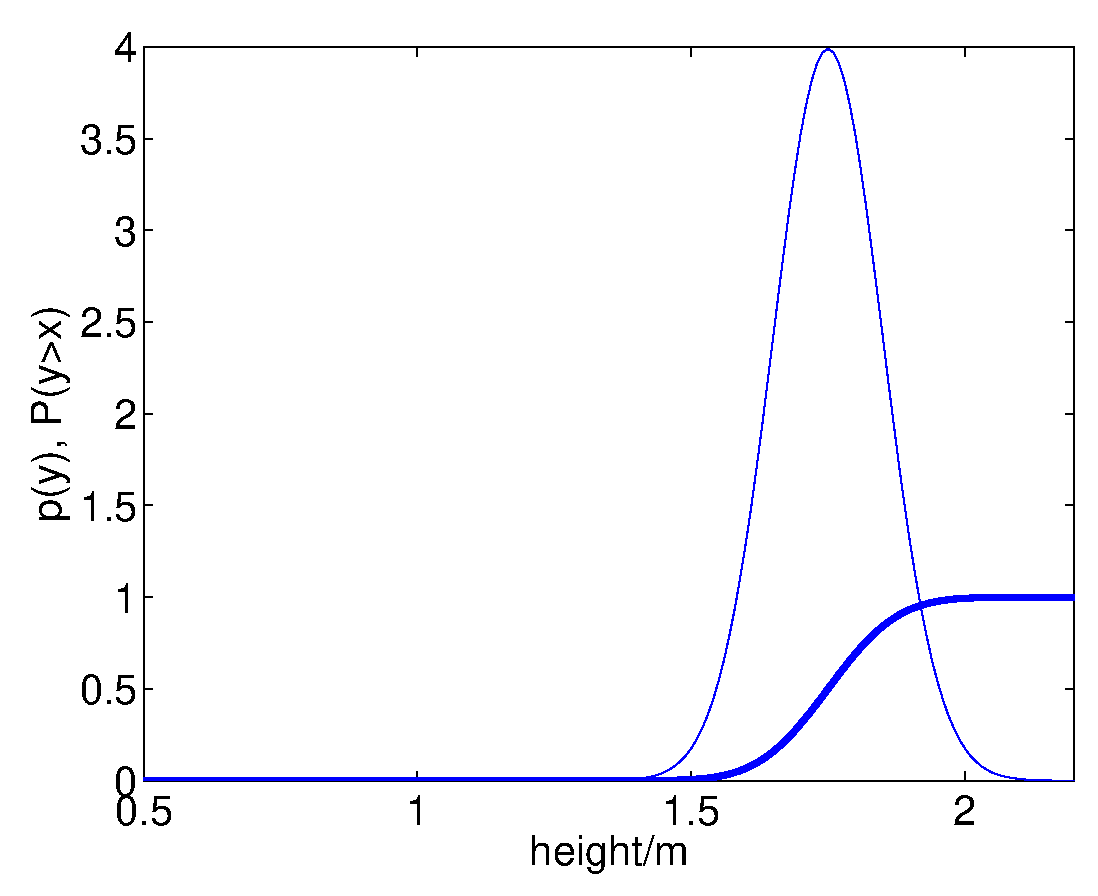
\includegraphics[%
  scale=0.5]{diagrams/cdfOfHeight.eps}\end{center}


\caption{The cummulative distribution function (CDF) for the heights of MSc
students. The thick curve gives the CDF and the thinner curve the
associated PDF.}
\end{figure}


Finally, we note that since the cummulative density function is the
integral of the probability density function the PDF can be recovered
from the CDF through differentiation.


\rotatefoilhead[-0.5in]{Sample Based Approximations}

Recall from Section~\ref{sec:expectations} that expectation of any
given function, $f\left(k\right)$, under a distribution, $P\left(k\right)$,
can be written as \[
\left\langle f\left(k\right)\right\rangle _{P\left(k\right)}=\sum_{k}f\left(k\right)P\left(k\right)\]
which is also written as $E\left\{ f\left(k\right)\right\} $. Recall
our definition of probability from Section~. \[
P\left(k\right)=\lim_{S\rightarrow\infty}\frac{s_{k}}{S}\]
where we have now used $S$ (instead of $N$) as the total number
of samples or trials from a system and $s_{k}$ is the number that
have state $k$. When we make \emph{sample based approximations} we
hope that $S$ is `large enough%
\footnote{How large $S$ need be is dependent on both the function whose expecation
we are estimating and and the distribution under which we are taking
the expectation.%
}' such that it is a good approximation to say\[
\left\langle f\left(k\right)\right\rangle _{P\left(k\right)}\approx\sum_{k}f\left(k\right)\frac{s_{k}}{S}.\]
This formula may be rewritten as:\[
\sum_{k}f\left(k\right)\frac{s_{k}}{S}=\frac{1}{S}\sum_{k}f\left(k\right)s_{k}.\]
Now if $\mathbf{k}$ is a vector of samples from $P\left(k\right)$with
elements $k_{i}$ and length $S$ then we can rewrite the above\[
\frac{1}{S}\sum_{k}f\left(k\right)s_{k}=\frac{1}{S}\sum_{i=1}^{S}f\left(k_{i}\right)\]
which provides us with a sample based approximation to the true expectation:
\[
\left\langle f\left(k\right)\right\rangle _{P\left(k\right)}\approx\frac{1}{S}\sum_{i=1}^{S}f\left(k_{i}\right).\]
Some well know special cases of this include the \emph{sample mean,}
often denoted by $\bar{k}$, and computed as\[
\bar{k}=\frac{1}{S}\sum_{i=1}^{S}k_{i},\]
this sample based mean is an approximation to the true distribution
mean\[
\left\langle k\right\rangle \approx\bar{k}.\]
The same approximations can be used in the context of continuous PDFs,
so we have\begin{eqnarray*}
\left\langle f\left(x\right)\right\rangle _{p\left(x\right)} & = & \int f\left(x\right)p\left(x\right)dx\\
 & \approx & \frac{1}{S}\sum_{i=1}^{S}f\left(x_{i}\right),\end{eqnarray*}
where $x_{i}$ are independently obtained samples from the distribution
$p\left(x\right)$.

The approximation gets better for increasing $S$ and worse if the
samples from $P\left(k\right)$ are \emph{not} independent.


\rotatefoilhead[-0.5in]{Sample Means for Student Heights}

Returning to our example concerning the height of MSc students, since
we don't know the true underlying distribution of MSc students, $p\left(h\right)$,
we cannot compute the mean of the distribution, but we can approximated
it with the sample mean: so if we want the mean, $f\left(h\right)=h$,
since we can't compute\[
\int_{0}^{\infty}hp\left(h\right)dh=\frac{1}{S}\sum_{i=1}^{S}f\left(k_{i}\right).\]
In most texts the word mean is used interchangeably to describe sample
based means and the true mean of a distribution. However, you should
always bear in mind the important difference between the two. Later
in the course we will also come across time based averages and assumptions
will be made that the time based average is equal to the average under
a steady state distribution.

\textbf{\emph{}}


\rotatefoilhead[-0.5in]{Poisson Processes}

In Section~\ref{sec:distributionAsFunction} we introduced probability
distributions that were dependent on functions. In this Chapter we
will introduce probabilistic processes. 


\rotatefoilhead[-0.5in]{Stochastic Processes}

A probabilistic process, also known as a random process or a stochastic
process, can be viewed as a `random function'. A normal function maps
a set of inputs to a point value. A probabilistic process maps a set
of inputs to a probability distribution over values or a probability
density function.

Various systems are modelled with probabilistic processes. For example,
the \emph{Wiener process} is the process behind Brownian motion. Stock
market data is often modelled as a stochastic process. For example
the Black-Scholes formula assumes that the logartihm of the stock
market data can be modelled as a Wiener Process.

We will base our definition of a random process on that given by \cite{Chan:performance00}.

\begin{description}
\item [A~random~process]may be defined as a \emph{random function} which,
for a particular value, is a random quantity. 
\end{description}

\rotatefoilhead[-0.5in]{Poisson Process}

We've already met the Poisson distribution, there is a simple process
which is related to the Poisson distribution: the Poisson process.

The Poisson process gives probabilities of a number of arrivals, $k$,
as a function of time, $t$, given a `rate', $\lambda$. 

\begin{equation}
P\left(k|t,\lambda\right)=\frac{(\lambda t)^{k}}{k!}e^{-\lambda t}.\label{eq:process}\end{equation}
Note the similarity between (\ref{eq:poissonDist}) and (\ref{eq:process}).
The process is simply the distribution with $\mu$ substituted with
$\lambda t$. The parameter $\lambda$ is now known as a rate, because
the product $\lambda t$ gives the expected number of arrivals at
time $t$.

By this substitution the mean of the Poisson process (the first moment
of $k$) is given by\[
\left\langle k\right\rangle =\lambda t.\]
Which is the expected number of arrivals at a given time $t$ if the
rate of the process is $\lambda$. The Poisson process is a form of
counting process where the counts are expected to increase linearly
with time. 


\rotatefoilhead[-0.5in]{Properties}

In the next few lectures we will derive the Poisson process from some
simple assumptions about how arrivals occur, for the moment we will
highlight some important properties of the Poisson process.


\rotatefoilhead[-0.5in]{Superposition of Poissons}

The first property we will consider is superposition of Poisson flows.
It is a property of a Poisson process that if we combine $N$ independent%
\footnote{Two variables $x$ and $y$ are independent if their joint distributions
are equal to the product of their marginal distributions $P\left(x,y\right)=P\left(x\right)P\left(y\right)$.%
} processes with rates $\lambda_{1},\lambda_{2},\dots,\lambda_{N}$
together the resulting process is also a Poisson process with a combined
rate, $\lambda$, equal to the sum of each of the input rates: $\lambda=\sum_{n=1}^{N}\lambda_{n}$.
This is shown pictorially in Figure~\ref{cap:poissonSuperposition}.

%
\begin{figure}[ht]
\begin{center}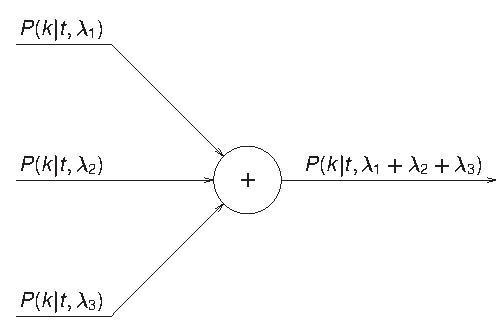
\includegraphics{./diagrams/sumPoisson.eps}%~\vspace{8cm}
\end{center}


\caption{If independent Poisson processes form a single traffic flow the rate
of the overall process is the sum of the separate processes.\label{cap:poissonSuperposition}}
\end{figure}


\begin{minipage}[c]{1.0\columnwidth}%
~


\rotatefoilhead[-0.5in]{Example of Poisson Superposition}


\rotatefoilhead[-0.5in]{Question }

There are three queues for registration of MSc students from different
courses at the University of Sheffield. Students for the first course,
Physics and Fine Art, arrive with a rate of 4 students per minute.
Students for the second course, The Psychology of Sociology, arrive
with a rate of 2 students per minute and students for the third course,
Computer Science and Aromatherapy arrive with a rate of 5 students
a minute.

Assuming the student arrivals are independent and occur as a Poisson
process what is the probability that after 15 minutes there have been
\textbf{a)} 90 student arrivals? \textbf{b)} 180 arrivals?


\rotatefoilhead[-0.5in]{%/*~\vspace{10cm}
Answer}

If the arrivals are indpendent and occur as a Poisson process, the
rate of arrivals for all student is the sum of the rates for each
course. $\lambda=4+2+5=11$. Now we simply evaluate (\ref{eq:process})
with $t=15$, $\lambda=11$ and \textbf{a)} $k=90$ giving \[
P\left(k=90|\lambda=11,t=15\right)=\frac{\left(11\times15\right)^{90}}{90!}\exp\left(-\left(11\times15\right)\right)=5.5\times10^{-11}.\]
and \textbf{b)}

\[
P\left(k=90|\lambda=11,t=15\right)=\frac{\left(11\times15\right)^{180}}{180!}\exp\left(-\left(11\times15\right)\right)=?.\]


Now ask someone with a calculator to work this out. Factorial 180
will definitely not work. Explain that it needs to be computed as:

\[
P\left(k=90|\lambda=11,t=15\right)=\exp\left(180\times\ln\left(11\times15\right)-\ln\left(180!\right)-\left(11\times15\right)\right)=0.015.\]
%~*/


~\end{minipage}%



\rotatefoilhead[-0.5in]{Decomposition of Poisson Flow}

Just as Poisson processes can be combined to obtain a higher rate
Poisson process, they can also be decomposed to obtain lower rate
Poisson processes with lower rates. Assume we have one input channel
where arrivals are occuring with a Poisson process with rate $\lambda$.
This channel then splits into $N$ separate output channels. Each
input arrival is then independently assigned to output channel $n$
with probability $P\left(n\right)$. In this case the output channels
then behave like Poisson processes with rates given by $\lambda_{n}=P\left(n\right)\lambda$.
This is shown in Figure~\ref{cap:decompositionPoisson}.

%
\begin{figure}[ht]
\begin{center}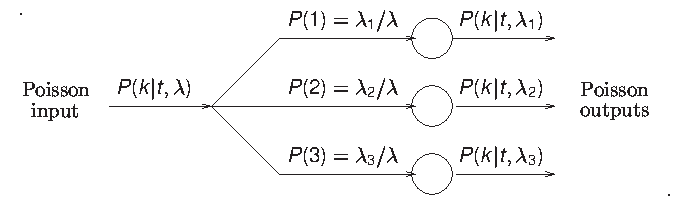
\includegraphics{./diagrams/decomposePoisson.eps}%~\vspace{8cm}
\end{center}


\caption{If a single Poisson process with rate $\lambda$ is switched to different
output channels, with each arrival being switched to channel $n$
with probability $P\left(n\right)=\lambda_{n}/\lambda$, each output
channel will be a Poisson process with rate $\lambda_{n}$.\label{cap:decompositionPoisson}}
\end{figure}


\begin{minipage}[c]{1.0\columnwidth}%
~


\rotatefoilhead[-0.5in]{Example of Poisson Decomposition}


\rotatefoilhead[-0.5in]{Question }

There is one registration for all MSc courses. Students arrive in
the hall and are assigned to registration desks according to the first
letter of their surname. Desk 1 ($d=1)$takes students with names
from A-G, desk 2 ($d=2$) from H-M, desk 3 ($d=3$) from N to S and
desk 4 ($d=4$) from R to Z. 

Surnames are distributed amoungst these four categories with the following
probability distribution:

\begin{center}\begin{tabular}{|c|c|c|c|c|}
\hline 
$d$&
1&
2&
3&
4\tabularnewline
\hline
\hline 
$P\left(d\right)$&
$0.20$&
$0.27$&
$0.25$&
$0.28$\tabularnewline
\hline
\end{tabular}\end{center}

Assuming the students arrive independently of their surname as a Poisson
process at a rate of 10 students per minute what is the probability
lity that \textbf{a)} after 5 minutes 5 students have arrived at desk
1? \textbf{b)} after 10 minutes 20 students have arrived at desk 4?


\rotatefoilhead[-0.5in]{%/*~\vspace{10cm}
Answer}

If the splitting is indpendent of the arrival, then the arrivals at
each desks will also occur as a Poisson process. For \textbf{a)} arrivals
at \textbf{}desk 1 will occur as a Poisson process with rate $\lambda_{1}=0.20\times10=2$.
The probability that $k=5$ students will have arrived at desk 1 after
$t=5$ minutes is given by substituting these values into (\ref{eq:process}):
\[
P\left(k=5|\lambda_{1}=2,t=5\right)=\frac{\left(2\times5\right)^{5}}{5!}\exp\left(-\left(2\times5\right)\right)=0.038.\]
For \textbf{b)} arrivals at \textbf{}desk 4 will occur as a Poisson
process with rate $\lambda_{4}=0.28\times10=2.8$. The probability
that $k=20$ students will have arrived at desk 1 after $t=10$ minutes
is again given by substituting these values into (\ref{eq:process}):
\[
P\left(k=20|\lambda_{4}=2.8,t=10\right)=\frac{\left(2.8\times10\right)^{20}}{20!}\exp\left(-\left(2.8\times10\right)\right)=0.025.\]
%~*/


~\end{minipage}%



\rotatefoilhead[-0.5in]{Independence of Arrivals\label{sub:poissonIndependence}}

Consider a single Poisson process, if we look within this process
at two \emph{disjoint} time intervals (\emph{i.e.} periods of time
that don't overlap). Assume we have $k_{1}$ arrivals in the first
interval and $k_{2}$ arrivals in the second interval. The distribution
of arrivals in the two intervals are independent of each other, $P\left(k_{1},k_{2}\right)=P\left(k_{1}\right)P\left(k_{2}\right)$. 


\rotatefoilhead[-0.5in]{Similarity of Arrival Distributions for Identical Intervals\label{sub:poissonSimilarities}}

Consider a single Poisson process with rate $\lambda$, let the number
of arrivals between time $s$ and $s+t$ be given by $k_{1}$. Now
consider a second independent Poisson process with the same rate $\lambda$,
let the number of arrivals between time $r$ and $r+t$ be given by
$k_{2}$. The distribution of $k_{1}$ and $k_{2}$ are then equal,
\[
P\left(k_{1}\right)=P\left(k_{2}\right).\]
 


\rotatefoilhead[-0.5in]{Interarrival Times and Poisson Processes}

The Poisson process is a simple model of arrivals that is widely used
due to its analytical properties. We have already seen how a superpositions
and decompositions of Poisson processes also lead to Poisson processes.
Another attractive analytical property is the ease with which we can
compute the \emph{interarrival time distribution} for the Poisson
process. 

The interarrival time distribution is the distribution of times between
arrivals. Consider waiting for the next bus at a bus stop. If you
just missed a bus how long will you have to wait for the next bus
to arrive? If the buses arrive as a Poisson process, then it is straightforward
to work out the distribution of these times.

%
\begin{figure}[ht]
\begin{center}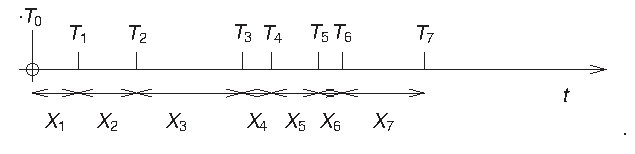
\includegraphics{./diagrams/interArrivals.eps}\end{center}


\caption{For a Poisson process, this figure shows the times of the arrivals,
$T_{n}$, and the interarrival times, $X_{n}$.\label{cap:poissonInterArrival}}
\end{figure}


In Figure~\ref{cap:poissonInterArrival} we show different arrival
times, $T_{1},\dots,T_{n}$ for the process. You can think of these
at the arrival times of the buses. We are interested in computing
the distribution of the variables $X_{i}=T_{i}-T_{i-1}$: the times
between bus arrivals. In the next section we will derive this PDF
for the interarrival times%
\footnote{The interarrival times, $X_{i}$, are continuous values, so they will
be governed by a probability density function rather than a discrete
probability distribution.%
}.


\rotatefoilhead[-0.5in]{Derivation of Interarrival Time Distribution}

Firstly we define the number of arrivals at time $t$ to be given
by the function $N\left(t\right)$. Next we note that the cumulative
density function (CDF) of the interarrival time distribution will
be given by $P\left(X_{i}\leq t\right)$ (see Section~\ref{sub:CDFs}
for a reminder on CDFs). We can re-write this probability as\[
P\left(X_{i}\leq t\right)=1-P\left(X_{i}>t\right),\]
so, rather than focussing on $P\left(X_{i}\leq t\right)$, we can
consider the distribution $P\left(X_{i}>t\right)$. Now we rewrite%
\footnote{The `$\equiv$' sign should be read as `is equivalent to'.%
} this condition in this distribution as\begin{eqnarray}
\left(X_{i}>t\right) & \equiv & \left(T_{i}-T_{i-1}>t\right)\nonumber \\
 & \equiv & \left(T_{i}>T_{i-1}+t\right),\label{eq:conditionInterarrival}\end{eqnarray}
where we have simply used the definition of $X_{i}$ and rearranged
the inequality. Let's take the time that $T_{i-1}$ occurs to be $t_{i-1}$.
This lets us write the condition (\ref{eq:conditionInterarrival})
as $\left(T_{i}>T_{i-1}+t|T_{i-1}=t_{i-1}\right)$. This will be true
if and only if the function $N\left(t\right)$ does not change during
the interval $\left(t_{i-1},t_{i-1}+t\right)$. We can express this
mathematically as \[
\left(X_{i}>t|T_{i-1}=t_{i-1}\right)\equiv\left(N\left(t_{i-1}+t\right)-N\left(t_{i-1}\right)=0\right).\]
The right hand side of this statement expresses the condition that
no arrivals occur between time $t_{i-1}=T_{i-1}$ and time $t$. 

\[
P\left(X_{i}>t|T_{i-1}=t_{i-1}\right)=P\left(N\left(t_{i-1}+t\right)-N\left(t_{i-1}\right)=0\right)\]
now, because of the similarity of the arrival distributions for intervals
of identical lengths (Section~\ref{sub:poissonSimilarities}) we
can write\[
P\left(N\left(t_{i-1}+t\right)-N\left(t_{i-1}\right)\right)=P\left(N\left(t\right)\right)\]
which means that\[
P\left(N\left(t_{i-1}+t\right)-N\left(t_{i-1}\right)=0\right)=P\left(N\left(t\right)=0\right)\]
and substituting $N\left(t\right)=k=0$ into (\ref{eq:process}) we
find that the probability of their being no arrivals at time $t$,
$P\left(N\left(t\right)=0\right)$, is \[
P\left(N\left(t\right)=0\right)=\exp\left(-\lambda t\right)\]
so\[
P\left(X_{i}>t\right)=\exp\left(-\lambda t\right)\]
and the CDF we are interested in is given by \begin{eqnarray*}
P\left(X_{i}\leq t\right) & = & 1-P\left(X_{i}>t\right)\\
 & = & 1-\exp\left(-\lambda t\right).\end{eqnarray*}
Now to obtain the PDF we simply differentiate the CDF (Section~\ref{sub:CDFs})
giving\[
p\left(X_{i}\right)=\lambda e^{-\lambda X_{i}}\]
which is the interarrival time distribibution. The form of the distribution
is recognised as an \emph{exponential distribution}. The parameter
of the exponential, $\lambda$, is the rate parameter from the Poisson
process.

In this section we have outlined the proof that the interarrival times
for a Poisson process are distributed exponentially. Hereafter, we
will use these formulations interchangeably, \emph{i.e.} when we state
that the interarrival times for students registring at the Goodwin
Sports centre is given by an exponential distribution with parameter
$\lambda=2$ we are equivalently stating that these students are arriving
according to a Poisson process with rate parameter $\lambda=2$.

\begin{minipage}[c]{1.0\columnwidth}%

\rotatefoilhead[-0.5in]{Consequences of Exponential Interarrival Times}

Let's assume that buses wait Waiting for a bus that arrives as a Poisson
process ... you are more likely to arrive in a longer interval than
a short one ... also it doesn't matter when you turn up, your expected
wait never changes .. this is the memoryless property of the exponential.\end{minipage}%



\rotatefoilhead[-0.5in]{Properties of the Exponential Distribution}


\rotatefoilhead[-0.5in]{The Memoryless property}

We have already seen in our derivation of the exponential as interarrival
time distribution that it is \emph{memoryless}. Formally speaking
this means that for exponentially distributed variable $X$\[
P\left(X>s+t|X>t\right)=P\left(X>s\right)\]
or in English, the probability of the waiting time being greater than
$s+t$ given that the waiting time is already greater than $t$ is
the same as the probability of the waiting time being greater than
$s$.


\rotatefoilhead[-0.5in]{Mean and Variance}

Recall the exponential distribution \[
p(x)=\lambda e^{-\lambda x}\]
 The mean of an exponential can be found to be, \[
\left\langle x\right\rangle _{p(x)}=\frac{1}{\lambda}\]
 and the variance is \[
\left\langle x^{2}\right\rangle _{p(x)}-\left\langle x\right\rangle _{p(x)}^{2}=\frac{1}{\lambda^{2}}.\]
 These are easily confirmed --- try doing them in your free time! 


\rotatefoilhead[-0.5in]{Markov Chains and Markov Processes}

In the last Chapter we introduced the Poisson process. In this chapter
we will show how the Poisson process in a special case of the more
general class of processes known as Markov processes. We will start
by considering Markov processes as they operate in \emph{discrete
time}, otherwise known as \emph{Markov chains}. Both Markov processes
and Markov chains exhibit the \emph{Markov property} which is an assumption
about how future values drawn from the process depend on past values.
We will first discuss the Markov property in the context of Markov
chains, then we will show how a discrete system can be converted to
a continuous system.


\rotatefoilhead[-0.5in]{Markov Chains}

Time is a continuous variable, but sometimes it is convenient, or
natural, to discretise time. One example of a form of discretised
time would be turns in a board game. As the turns progress this discretised
form of time progresses.

Consider a discrete representation of time $t=0,1,2...$. We associate
a state variable, $N$, with this time such that we have values for
$N$ at $N(0),\, N(1),\, N(2),\,...$. 


\rotatefoilhead[-0.5in]{Markov Property}

If this state variable exhibits the Markov property its value at time
$t$ is dependent only on its value at time $t-1$. The common way
of putting this property is that the future is conditional independent
of the past. The conditioning being on the present. In other words,
the state of the system in the future is \emph{not} dependent on what
happened in the past if we know the state at the present time.

Let's consider a real-life example of a Markov chain, that of the
board game of Monopoly.


\rotatefoilhead[-0.5in]{Monopoly Board }

There are forty squares on a Monopoly board. We assume that there
is only one player. That player's state, $N(t)$, will be the number
of the square his/her counter is on $+40$ for every time he/she has
reached GO. For example if you have circled the board twice and are
currently on GO then $N(t)=80$. Or if you have circled the board
once and are on King's Cross then $N(t)=45$. The time $t$ is now
clearly discrete and associated with the number of turns the player
has had. 

In Monopoly you move your counter through rolling two six sided dice
and adding them together. We will denote the result of this die roll
at time $t$ with $d(t)$. Notice that your state after turn $t$,
$N(t)$ depends only on your die role, $d(t)$, and your state before
turn $t$, $N(t-1)$. We write this as: \[
N(t)=N(t-1)+d(t).\]
 This means that Monopoly exhibits the Markov property, as your future
states are independent of your previous states given your current
state.


\rotatefoilhead[-0.5in]{State Diagrams}

A Markov chain can be represented by a state diagram just as finite
state machines are often represented in this manner. One important
difference is that Markov chains are not necessarily finite, they
can have infinity states! A further difference is that the transitions
for Markov chains are associated with probabilities (or in the case
of Markov processes rates).

%
\begin{figure}[ht]
\begin{center}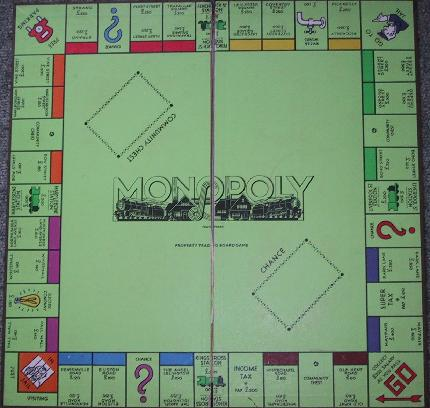
\includegraphics{diagrams/smallMonopoly.jpg}\end{center}


\caption{Image of a monopoly board.}
\end{figure}



\rotatefoilhead[-0.5in]{Poisson Process as a Markov Process}

We've introduced the game of Monopoly as a Markov chain. In this next
session we shall relate Markov chains, where time is treated as a
discrete variable, to Markov processes, where time is a continuous
variable. We will show how the Poisson process is a special case of
a Markov process where a constrained set of transitions are allowed.
To do this we will first introduce a new version of Monopoly that
we call `Coin Monopoly'. 


\rotatefoilhead[-0.5in]{Coin Monopoly}

In regular Monopoly each jump, $d(t)$, is given by the sum of two
die rolls. Let's assume that we have Monopoly addicts but we have
lost the dice for our set of Monopoly. In danger of going into withdrawl
and, finding a coin in our pocket, we come up with the following way
of playing the game.

In the coin version of Monopoly each player tosses the coin when it
is their turn. Then, instead of $d(t)$ being the sum of two die roles,
we take $d(t)=0$ if a coin is tails and $d(t)=1$ if it is heads.
This is depicted as a state diagram in Figure~\ref{cap:coinMonopolyStateDiagram}. 

Now lets consider one addict, Anne, who enjoys this version of the
game so much that she decides to play it on her own. Unfortunately
there is one drawback to playing in this way: it takes rather a long
time. However, Anne is a keen mathematician and tries to find a way
of speeding it up. 

Currently, with each turn, we consider time, $t$, to change by $\Delta t=1$.
Let's pretend we have a special coin where we can change the probability
that it will be heads. We denote this probability, $P\left(h\right)=\lambda\,\Delta t$
(which must be less than 1), giving $P\left(t\right)=1-\lambda\,\,\Delta t$.
%
\begin{figure}[ht]
\begin{center}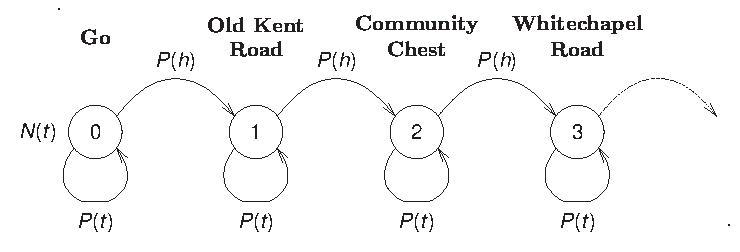
\includegraphics{./diagrams/stateDiagram.eps}\end{center}


\caption{State diagram for coin monopoly. Each circle represents a different
possible state value. The state changes (or doesn't change) with each
time step according the probabilities associated with the arrows.
\label{cap:coinMonopolyStateDiagram}}
\end{figure}


Anne can now compute the probability that, after $n$ turns, the state
of the system will be $k$ using the \emph{binomial distribution}.


\rotatefoilhead[-0.5in]{Binomial Distribution for $n$ Trials}

Consider a system with two states (such as a coin). Let's assume that
one of those states is associated with `success' and one is associated
with `failure'. In our Coin Monopoly example heads might be considered
success (because it is associated with a move forward) and tails might
be associated with failure (because it is associated with no move). 

It is possible to compute a probability distribution for a number
of successes given a number of trials. This distribution is known
as the binomial. For $n$ trials (equivalent to $n$ coin tosses or
$n$ turns for Coin Monopoly) the probability of $k$ successes (equivalent
to $k$ moves forward) is given by 

\begin{equation}
P\left(k\right)=\left(\begin{array}{c}
n\\
k\end{array}\right)P\left(h\right)^{k}(1-P\left(h\right))^{n-k}\label{eq:binomialDistirbution}\end{equation}
where $\left(\begin{array}{c}
n\\
k\end{array}\right)=\frac{n!}{k!(n-k)!}$ is known as the binomial coefficient. 

Since each of our turns takes $\Delta t$ time, we know that after
$t$ time we will have completed \begin{equation}
n=\frac{t}{\Delta t}\label{eq:nInTermsOfDeltaT}\end{equation}
 turns. Since we defined $P\left(h\right)=\lambda\Delta t$ we can
therefore write\[
P\left(h\right)=\frac{\lambda t}{n}.\]
We now substitute this expression for the probability of heads into
the binomial distribution (\ref{eq:binomialDistirbution}) giving
\begin{eqnarray*}
P\left(k|\lambda,t\right) & = & \frac{n!}{k!(n-k)!}\left(\frac{\lambda t}{n}\right)^{k}\left(1-\frac{\lambda t}{n}\right)^{n-k}\\
 & = & \frac{n\left(n-1\right)\dots\left(n-\left(k-1\right)\right)}{n^{k}\left(1-\frac{\lambda t}{n}\right)^{k}}\frac{(\lambda t)^{k}}{k!}\left(1-\frac{\lambda t}{n}\right)^{n}.\end{eqnarray*}
The next step is to take the limt as $n\rightarrow\infty$. From (\ref{eq:nInTermsOfDeltaT})
we can see that this is equivalent to equivalent to taking $\Delta t\rightarrow0$.
In this limit we can take advantage of the following \[
\lim_{n\rightarrow\infty}\frac{n\left(n-1\right)\dots\left(n-\left(k-1\right)\right)}{n^{k}\left(1-\frac{\lambda t}{n}\right)^{k}}=1.\]
You should recognise this from the fact that the dominant term in
the numerator is $n^{k}$ and the dominant term in the denomiator
is $n^{k}$. Secondly we use the fact that \[
\lim_{m\rightarrow\infty}\left(1+\frac{z}{m}\right)^{m}=\exp\left(z\right).\]
Inserting these two limits into the equation gives: \begin{equation}
P\left(k|\lambda,t\right)=\frac{(\lambda t)^{k}}{k!}e^{-\lambda t}.\label{eqn:poisson}\end{equation}
which is recognised as a Poisson process. In other words, we have
proved that a Poisson process is a particular type of Markov chain,
in fact, because we have taken the limit as $\Delta t\rightarrow0$,
this system is now continous time, it is therefore known as a Markov
process. 


\rotatefoilhead[-0.5in]{Markov Process State Diagrams}

When drawing state diagrams for continuous systems there a couple
of small differences to the Markov chain state diagram given in Figure~\ref{cap:coinMonopolyStateDiagram}.
We no longer include the arrows that point to the same state and we
replace the probability of state transfer with a rate of transfer
between states (see Figure~\ref{cap:coinMonopolyProcess}).

%
\begin{figure}[ht]
\begin{center}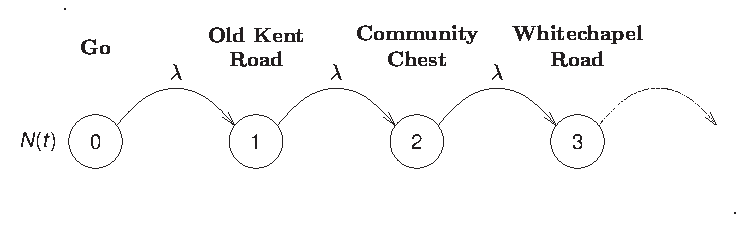
\includegraphics{diagrams/stateDiagramProcess.eps}\end{center}


\caption{State diagram for the Markov process given by Coin Monopoly in the
limit as $\Delta t\rightarrow0$. This is the state diagram for a
Poisson process. Notice in comparison to Figure~\ref{cap:coinMonopolyStateDiagram},
the probabilities have been replaced by rates and there are no self-transition
arrows.\label{cap:coinMonopolyProcess}}
\end{figure}
You've now seen that a Poisson process can be derived starting from
a simple Markov chain. This gives some deeper insight to a Poisson
process. In the coin monopoly model there is a fixed (constant) probability
of moving forward in every turn and whether a move forward occurs
in each turn is completely independent of what happened in previous
turns. The Poisson process is the continuous analoge of this stem.
There is a constant probability of an arrival occurring at any time
which is independent of what has gone before. This gives you an intuitive
explanation of the two properties of the Poisson process given in
Sections~\ref{sub:poissonIndependence}~and~\ref{sub:poissonSimilarities}. 


\rotatefoilhead[-0.5in]{Birth Death Processes and $M/M/1$ Queues}

A modification to our previous state diagram brings us to a birth-death
process. Imagine now that instead of tossing a coin, three possible
events may occur. The state may go up by one (a birth), down by one
(a death) or stay the same. 

We represent this with a state diagram as follows. 

%
\begin{figure}[ht]
\begin{center}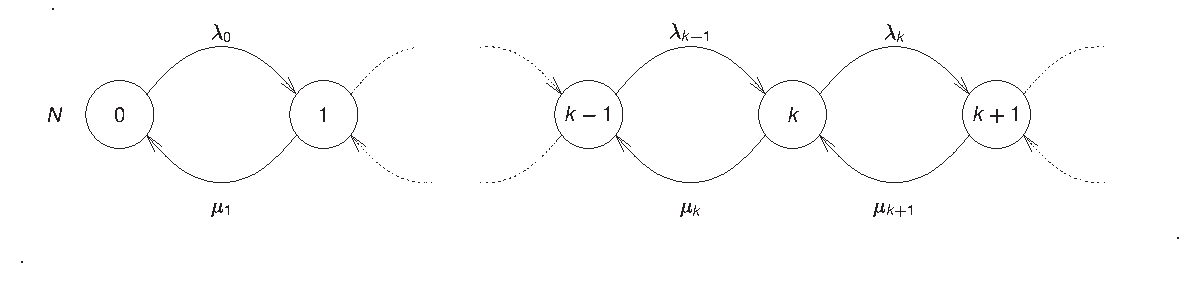
\includegraphics{./diagrams/birthDeathProcess.eps}\end{center}


\caption{State diagram for a birth-death process.}
\end{figure}


Such processes are ideal for modelling may types of queues. 


\rotatefoilhead[-0.5in]{M/M/1 Queue}

The M/M/1 queue represents a birth-death process where the birth rate
and death rate. 


\rotatefoilhead[-0.5in]{Kendall's Notation}

Arrival Distribution/Service Distribution/number of servers. 

$M$ - Markov/Memoryless, $G$ - General and $D$ - deterministic.


\rotatefoilhead[-0.5in]{Steady State Behaviour}

Often we are interested in the steady state behaviour of a system,
rather than the transient dynamics. We might ask the question what
is the average network delay when the system has reached steady state?
What do we mean by steady state? 

\begin{enumerate}
\item A stable condition that does not change over time or in which change
in one direction is continually balanced by change in another.%
\footnote{\texttt{http://www.dictionary.com}.%
}
\item A steady state is a dynamic equilibrium. 
\end{enumerate}
A Markov process, under certain conditions, will reach a steady state
distribution over $k$. Recall that a probabilistic process $p\left(k|t\right)$
is a `noisy function' of time. Some probabilistic processes will converge
to a probability distribution when we look at them in the limit as
time $\rightarrow\infty$. Not all will though, for example a Poisson
\emph{won't}.\[
\lim_{t\rightarrow\infty}p\left(k|t\right)=p\left(k\right)\]
the average value of $k$ at steady state is then given by\[
\left\langle k\right\rangle _{p\left(k\right)}=\sum_{k=0}^{\infty}p\left(k\right)k\]
in what follows we will assume that this steady state average is equivalent
to the time average in the limit as $t\rightarrow\infty$, where if
the state of the system is given as a function of time as $N\left(t\right)$
the average number in the system as a function of time is given by
\[
\bar{N}\left(t\right)=\frac{1}{t}\int_{0}^{t}N\left(\tau\right)d\tau\]
and the time average after in the limit as $t\rightarrow\infty$ is
given by \[
\bar{N}=\lim_{t\rightarrow\infty}\bar{N}\left(t\right).\]
which we assume is equivalent to $\left\langle k\right\rangle _{p\left(k\right)}\equiv\bar{N}$.
See pg 156-157 in Bertsekas and Gallager for more details. 


\rotatefoilhead[-0.5in]{Little's Formula}

Applies for $G$/$G$/1 queues. 

Little's formula gives the relationship between the steady-state average
size of a queue, $\bar{N}$, the steady-state arrival rate, $\lambda$,
and the steady-state customer delay, $\bar{T}$. 

Under steady state conditions, Little's formula states \[
\bar{N}=\lambda\bar{T}\]


Nightclub Queue. You are driving past a nightclub, wondering how long
you will have to wait to go in. You notice on Thursday nights the
queue typically contains 20 people and that people arrive at a rate
of 40 per hour. 

According to Little's formula, how long would you expect to have to
wait to get in? 

The waiting time is given by Little's formula. $\bar{N}=20$, $\lambda=40$
and $\bar{T}=\frac{\bar{N}}{\lambda}=\frac{20}{40}=\frac{1}{2}\textrm{hour}$. 


\rotatefoilhead[-0.5in]{Graphical Proof}

%
\begin{figure}[ht]
\begin{center}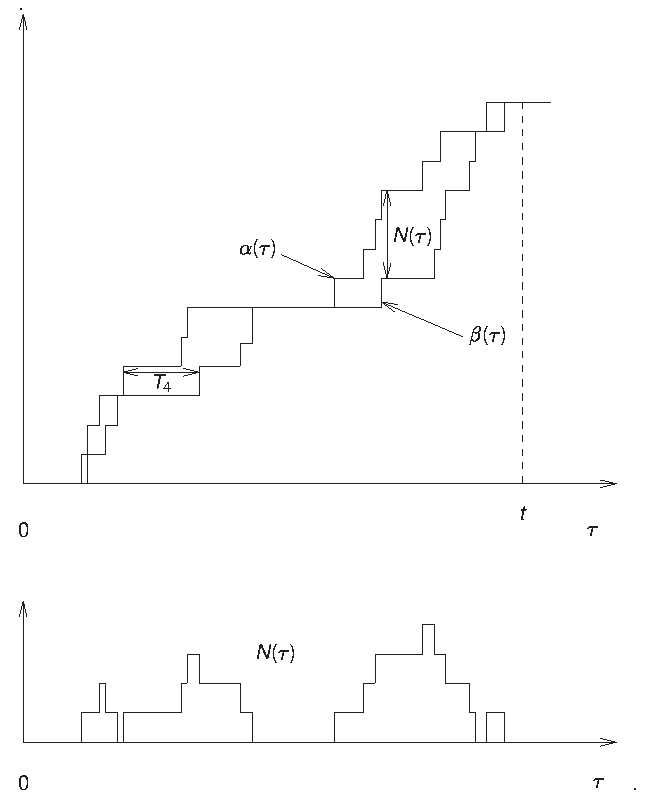
\includegraphics{./diagrams/littlesFormula.eps}\end{center}


\caption{Graphical `proof' of Little's formula.}
\end{figure}


The area between the lines in the top figure can be expressed as both
$\int_{0}^{t}N(\tau)d\tau$ and $\sum_{i=1}^{\alpha\left(t\right)}T_{i}$.
Dividing both expressions by $t$, equating them, and taking the limit
as $t\rightarrow\infty$ gives Little's formula. \[
\frac{1}{t}\int_{0}^{t}N(\tau)d\tau=\frac{1}{t}\sum_{i=1}^{\alpha(t)}T_{i}=\frac{\alpha(t)}{t}\frac{\sum_{i=1}^{\alpha(t)}T_{i}}{\alpha(t)}\]
 leading to \[
\bar{N}_{t}=\lambda_{t}\bar{T}_{t}\]
 We wish to consider the steady state behaviour. The system may not
have steady state behaviour. If the steady state exists, we can seek
it in the limit as $t\rightarrow\infty$, giving \[
\bar{N}=\lambda\bar{T}\]


This formula applies regardless of the arrival and service time distributions,
it only relies on the system being in steady state. 

Little's formula can be used at the system level, as we have seen,
or at a lower level. 


\rotatefoilhead[-0.5in]{Little's Formula for Queueing Time and Transmission Time }

The total delay for packet switching systems can be divided into queueing
time, $W$, and service time or transmission time, $X$. $T=X+W.$
Similarly the average delay may be divided. \[
\bar{T}=\bar{X}+\bar{W}\]
 

Both the queue itself and the transmission may be analysed independently
using Little's formula. 


\rotatefoilhead[-0.5in]{The Queue}

Given $\lambda$, an arrival rate, $\bar{N}_{Q}$, the average number
of packets waiting in the queue, and $\bar{W}$, the average packet
waiting time, Little's formula gives \[
\bar{N}_{Q}=\lambda\bar{W}.\]



\rotatefoilhead[-0.5in]{The Transmission}

For $\bar{X}$, the average transmission time, we can obtain the average
number of packets under transmission, \[
\rho=\lambda\bar{X},\]
 which is also known as the utilisation factor. It represents the
fraction of time that the transmission line is in use. For a $G/G/1$
queue it must be less than one, \emph{i.e.} arrival rate must be less
than $\frac{1}{\bar{X}}$. 

Note: time under transmission is often considered proportional to
packet length. For packet length of $L$ bits and bandwidth of $C$
bits per second transmission time is $X=\frac{L}{C}$. 

You are at a queue in a bar, and notice that the bar tender spends
10\% of her time cleaning between serving customers. If the typical
number of people waiting to be served is $3$, what is the ratio of
time spent waiting to being served? 

Information says $\rho=0.9$ and $\bar{N}_{Q}=3$. \[
\lambda=\frac{0.9}{\bar{X}}.\]


\[
3=\lambda\bar{W}.\]


Therefore $\frac{\bar{W}}{\bar{X}}=3\frac{1}{3}$. 


\rotatefoilhead[-0.5in]{$M$/$M$/1 Queue}


\rotatefoilhead[-0.5in]{Global Balance}

We seek a stationary distribution by looking for global balance equations.
Global balance equations state that at equilibrium the frequency of
transitions out of state $k$ equals the frequency of transitions
into $k$. (pg 260-262 Bertsekas and Gallager). 


\rotatefoilhead[-0.5in]{Discrete Time Markov Chain}

In its most general form a discrete time Markov process can be defined
by a transition probability matrix\[
\mathbf{P}=\left[\begin{array}{ccccc}
P_{11} & \cdots & P_{i1} & \cdots & P_{N1}\\
\vdots & \ddots &  &  & \vdots\\
P_{1j} &  & P_{ij} &  & P_{Nj}\\
\vdots &  &  & \ddots & \vdots\\
P_{1N} & \cdots & P_{iN} & \cdots & P_{NN}\end{array}\right]\]
if the steady state probability of being in state $j$ is $P\left(j\right)$
then the global balance equations state\[
P\left(j\right)\sum_{i=0}^{\infty}P_{ji}=\sum_{i=0}^{\infty}P\left(i\right)P_{ij}\]
which in English says the probability of leaving state $j$ is equal
to the probability of arriving in state $j$.


\rotatefoilhead[-0.5in]{Continuous Time Markov Chain}

In continuous time Markov chains we are interested in rates of transfer
rather than probabilities if the rates of transfer between states
are given by a matrix whose elements $q_{ij}$ give the rate of transfer
between state $i$ and state $j$, then the global balance equations
give\[
P\left(j\right)\sum_{i=0}^{\infty}q_{ji}=\sum_{i=0}^{\infty}P\left(i\right)q_{ij}.\]



\rotatefoilhead[-0.5in]{Detailed Balance}

For the birth death processes we are considering transitions only
occur between state $k$ and $k+1$ or $k-1$. This leads us to a
special case of the global balance equations known as the detailed
balance equations which look at the flow between two states. For the
discrete case\[
P\left(k-1\right)P_{k-1,k}=P\left(k\right)P_{k,k-1}\]
and for the continuous case \[
P\left(k-1\right)q_{k-1,k}=P\left(k\right)q_{k,k-1}\]
however in our notation the rate from $k$ to state $k-1$is given
by $\mu_{k}$ and the rate from $k-1$ to $k$ is given by $\lambda_{k-1}$.

%
\begin{figure}[ht]
\begin{center}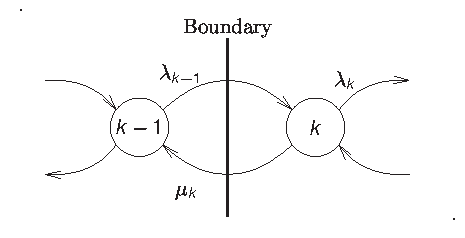
\includegraphics{./diagrams/boundaryFlow.eps}\end{center}


\caption{Flow rates at a Boundary.}
\end{figure}


Thus at steady state, flow from $k-1$ to $k$ = $\lambda_{k-1}P\left(k-1\right)$.
Flow from $k$ to $k-1$ is $\mu_{k}P\left(k-1\right)$. For flow
to be balanced we have \[
\lambda_{k-1}P\left(k-1\right)=\mu_{k}P\left(k\right)\]
 leading to \[
P\left(k\right)=\frac{\lambda_{k-1}}{\mu_{k}}P\left(k-1\right)\]
 


\rotatefoilhead[-0.5in]{$M$/$M$/$1$}

For the M/M/1 we assume that arrivals occur as a Poisson process,
and service times are exponentialy distributed. This implies a birth
death process with $\lambda_{k}=\lambda_{k-1}=\lambda$, $\mu_{k}=\mu_{k-1}=\mu$
giving \[
P\left(k\right)=\frac{\lambda}{\mu}P\left(k-1\right)\]
 Thus \begin{eqnarray*}
P\left(k\right) & = & \left(\frac{\lambda}{\mu}\right)^{k}\\
P\left(0\right) & = & \rho^{k}P\left(0\right),\end{eqnarray*}
 where we have defined $\rho=\frac{\lambda}{\mu}$, known as the utilisation
factor. 


\rotatefoilhead[-0.5in]{Normalisation}

We can find $P\left(0\right)$ by using the normalisation condition
$\sum_{k=0}^{\infty}P\left(k\right)=1$, therefore \[
1=P\left(0\right)\sum_{k=0}^{\infty}\rho^{k}\]
 Giving \[
P\left(0\right)=\frac{1}{\sum_{k=0}^{\infty}\rho^{k}}\]
 The series in the denominator converges if $\rho<1$ (when the birth
rate is less than the death rate), \[
\sum_{k=0}^{\infty}\rho^{k}=\frac{1}{1-\rho},\]
 meaning that \[
P\left(0\right)=\left(1-\rho\right)\]
 and allowing us to write down the \emph{steady state} probabilities.
\[
P\left(k\right)=\rho^{k}\left(1-\rho\right)\]



\rotatefoilhead[-0.5in]{Design Issues}

For the design of networks we are interested in the average queue
length (a design issue) and the average delay (a quality of service
issue). 

We can use the steady state probabilities, in combination with Little's
formula, to compute these quantities. 

Start by working out average number of customers in system (not the
same as average queue length). 

\begin{lyxcode}
\begin{eqnarray*}
\bar{N} & = & \left\langle k\right\rangle _{P\left(k\right)}\\
 & = & \sum_{k=0}^{\infty}kP\left(k\right)\\
 & = & \left(1-\rho\right)\sum_{k=0}^{\infty}k\rho^{k}\\
 & = & \rho\left(1-\rho\right)\sum_{k=0}^{\infty}k\rho^{k-1}\\
 & = & \rho\left(1-\rho\right)\frac{\partial\sum_{k=0}^{\infty}\rho^{k}}{\partial\rho}\\
 & = & \rho\left(1-\rho\right)\frac{\partial}{\partial\rho}\left[\frac{\rho}{1-\rho}\right]\\
 & = & \rho\left(1-\rho\right)\frac{1}{\left(1-\rho\right)^{2}}\\
 & = & \frac{\rho}{1-\rho}\\
 & = & \frac{\lambda}{\mu-\lambda}\end{eqnarray*}

\end{lyxcode}

\rotatefoilhead[-0.5in]{M/M/1 Queue - contd}

For the design of networks we are interested in the 

\begin{description}
\item [average~queue~length]a design issue 
\item [average~delay]a quality of service issue 
\end{description}
Last time Demo, steady state probabilities, average queue length. 

Other info --- the variance of the number in the system can be found
as \begin{equation}
\textrm{var}[k]=\left\langle k^{2}\right\rangle -\left\langle k\right\rangle ^{2}=\frac{\rho}{(1-\rho)^{2}}\end{equation}
 Confirm in your own time. 


\rotatefoilhead[-0.5in]{Review of Demo}

Show demo for high $\rho$ ($\lambda=1.8$,$\mu=2$) and low $\rho$
($\lambda=1$, $\mu=2$) exhibiting high $N$ and $T$ and low $N$
and $T$. Talk about how the probabilities converge to the steady-state
values, mention issues of heavy tails etc.. 

%
\begin{figure*}[ht]
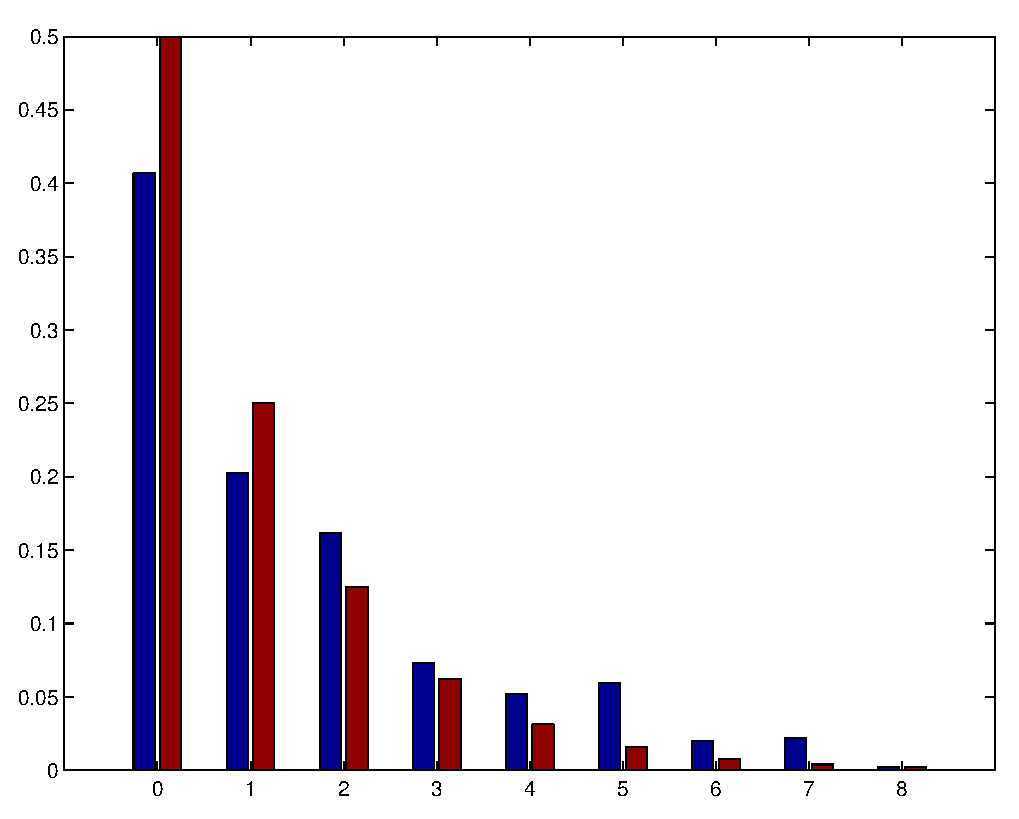
\includegraphics[%
  width=2.3622in]{diagrams/rho_half_100_arrivals.eps} \hfill{}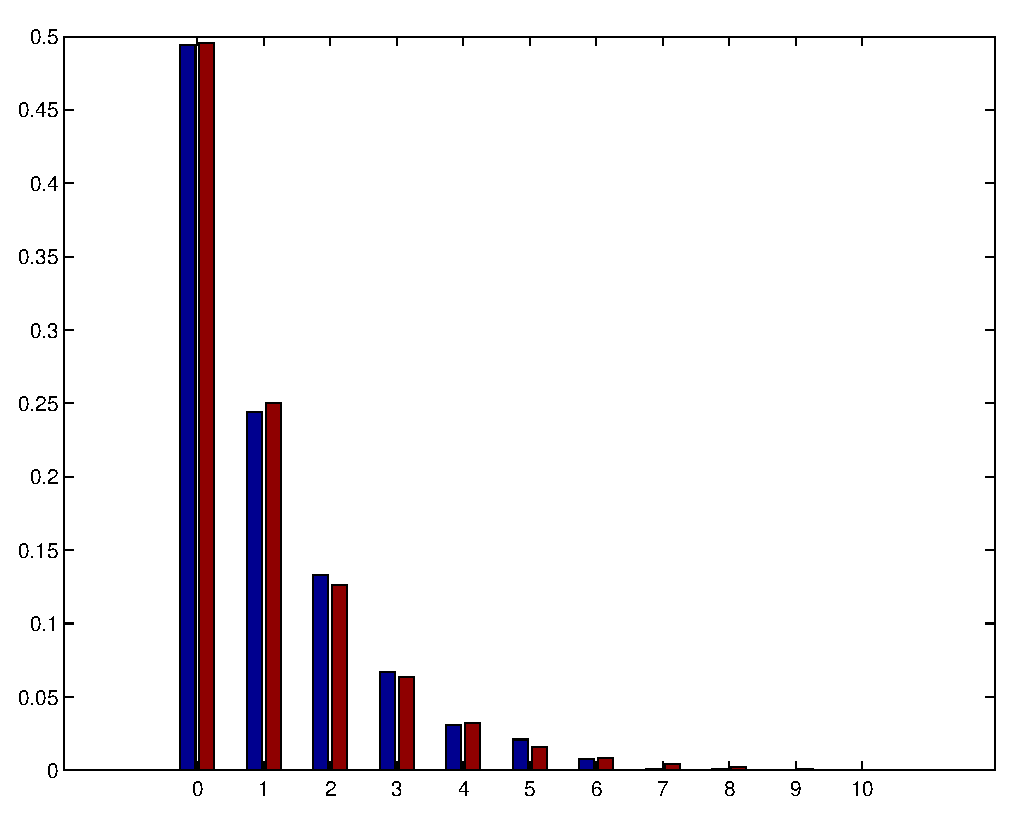
\includegraphics[%
  width=2.3622in]{diagrams/rho_half_1000_arrivals.eps}


\caption{Left figure: steady state probabilities after the first 100 seconds
for $\rho=0.5$. Right figue: steady state probabilities after the
first 1000 seconds for $\rho=0.5$.}
\end{figure*}


%
\begin{figure*}[ht]
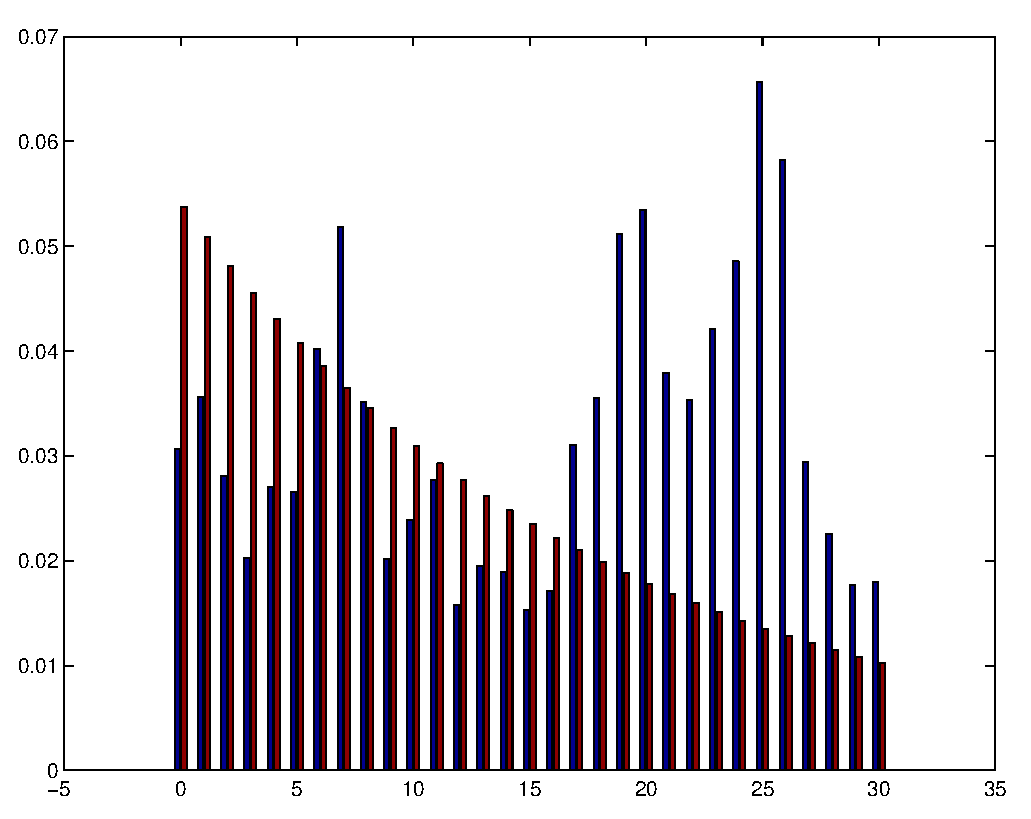
\includegraphics[%
  width=2.3622in]{diagrams/rho_point95_100_arrivals.eps} \hfill{}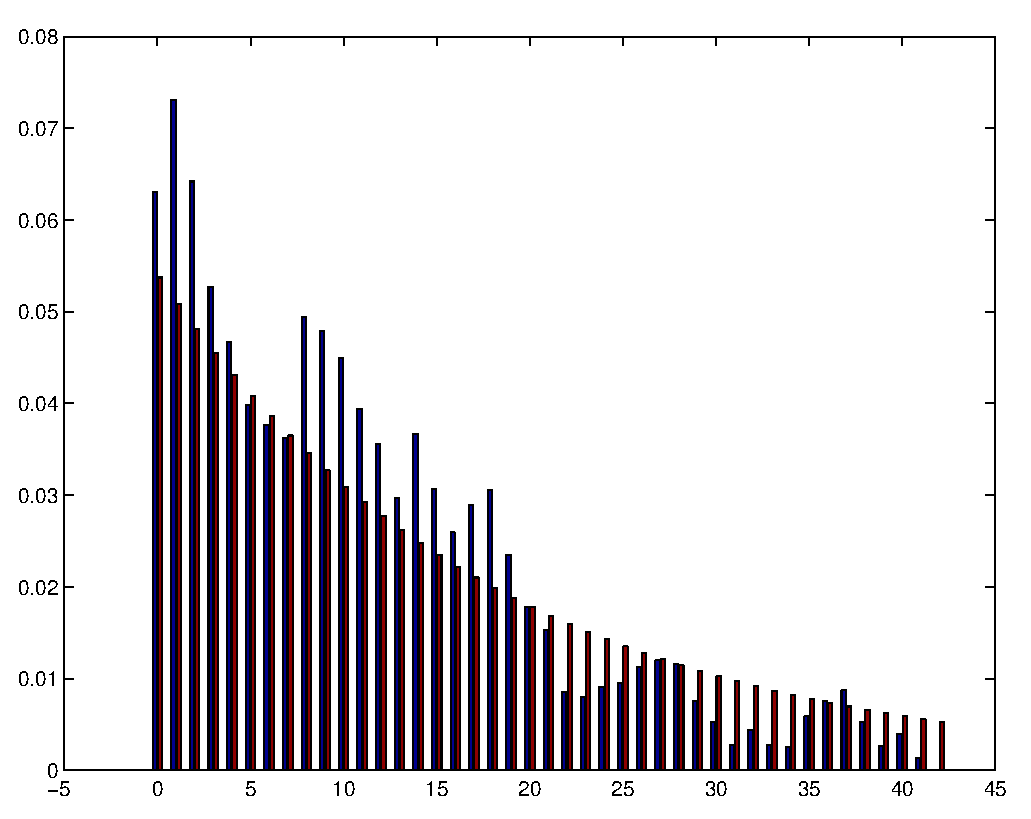
\includegraphics[%
  width=2.3622in]{diagrams/rho_point95_1000_arrivals.eps}


\caption{Left figure: steady state probabilities after the first 100 seconds
for $\rho=0.95$. Right figue: steady state probabilities after the
first 1000 seconds for $\rho=0.95$.}
\end{figure*}


If $n_{k}$ is the number of counts for each state after $n$ time
steps the approximation to the probability of each time step is $\frac{n_{k}}{n}$
where $\sum_{k=0}^{K}n_{k}=n$. 

Slide of steady state probabilities for $\rho$ close to 1. 


\rotatefoilhead[-0.5in]{Average Delay}

Little's formula tells us that $\bar{N}=\lambda\bar{T}$, where $\bar{T}$
is the average delay. This gives us the average delay as \[
T=\frac{1}{\mu-\lambda}\]
 This is not the time spent in the queue however, this is the time
spent in the system which includes \emph{propagation delay}. 


\rotatefoilhead[-0.5in]{Little's formula for Queue}

We can apply Little's formula again to find the number in the queue. 

The rate for this version is the same, but we are now interested in
the average number in the queue, $\bar{N}_{Q}$, the average waiting
time, $\bar{W}$, is given by \[
\bar{W}=\bar{T}-\frac{1}{\mu}=\frac{1}{\mu-\lambda}-\frac{1}{\mu}\]
 The rate of arrivals will be the same, so the average number in the
queue will be \[
\bar{N}_{Q}=\lambda\bar{W}=\frac{\rho^{2}}{1-\rho}\]



\rotatefoilhead[-0.5in]{Other Markov Queues}


\rotatefoilhead[-0.5in]{Statistical Multiplexing vs Time and Frequency division}


\rotatefoilhead[-0.5in]{Example 3.9 in Bertsekas \& Gallager}

Assume we have m statistically independent Poisson streams. Each has
arrival rate $\frac{\lambda}{m}$. Each has an average transmission
time $\bar{X}$. 

If we merge the Poisson streams together, through statisical multiplexing,
property of Poisson from Lecture 3\&4 tell us that they become a Poisson
stream with rate $\lambda$. Average delay, from last lecture will
be\[
\bar{T}=\frac{1}{\mu-\lambda}.\]
Now consider an alternative approach of providing each channel with
a seperate circuit. This involves splitting our transmission line
into $m$ channels. Each will now have bandwidth at most $\frac{\mu}{m}$.

Delay in this system will now be\[
\bar{T}=\frac{1}{\frac{\mu}{m}-\frac{\lambda}{m}}=\frac{m}{\mu-\lambda}\]
or $m$ times larger than statistical multiplexing. 

Why does this happen?

Consider the situtation where there is only one packet in the system.
In this case much of the bandwidth will be redundant.


\rotatefoilhead[-0.5in]{Kendall's notation}

Arrival Charateristics/Departure Charateristics/number of servers/maximum
number of customers


\rotatefoilhead[-0.5in]{Arrival and Departure Charateristics}

\begin{itemize}
\item $M$- Markov - Poisson distributed arrivals, exponentially distributed
service times.
\item $D$ - Deterministicly distributed times.
\item $G$ - General distribution for inter-arrival/service times.
\end{itemize}

\rotatefoilhead[-0.5in]{Finite Length $M$/$M$/$1$/$m$}

So far we have assumed that the queue can have an infinite length.
What if it has a restricted buffer of size $m$? 

Insert diagram here

Let us assume the queue can contain at maximum $m$ arrivals. The
balance equation from above still applies. However, now the normalisation
is different, giving a different value for $P\left(0\right)$. \[
\sum_{k=0}^{m}P\left(0\right)\rho^{k}=1\]
 Since this is simply a finite sum of a geometric series \[
P\left(0\right)=\frac{1}{\sum_{k=0}^{m}\rho^{k}}=\frac{1-\rho}{1-\rho^{m+1}}\]
 We therefore have \[
P\left(k\right)=\frac{\rho^{k}\left(1-\rho\right)}{1-\rho^{m+1}}\]


Given a finite length $M$/$M$/$1$/$m$ queue, what is the probability
that an arrival is blocked from joining the queue (and therefore lost). 

This is answered by determining the probability of the queue being
full, which means \[
P\left(m\right)=\frac{\rho^{m}\left(1-\rho\right)}{1-\rho^{m+1}}\]



\rotatefoilhead[-0.5in]{$M$/$M$/$\infty$}

Insert diagram here


\rotatefoilhead[-0.5in]{Detailed Balance }

\begin{eqnarray*}
\lambda_{k-1}P\left(k-1\right) & = & \mu_{k}P\left(k\right)\\
\lambda P\left(k-1\right) & = & k\mu P\left(k\right)\end{eqnarray*}
thus we can write\[
P\left(k\right)=\frac{\lambda}{k\mu}P\left(k-1\right)\]
and therefore\[
P\left(k\right)=P\left(0\right)\left(\frac{\lambda}{\mu}\right)^{k}\frac{1}{k!}\]
using the normalisation conditions we can see that\begin{eqnarray*}
\sum_{k=0}^{\infty}P\left(k\right) & = & 1\\
P\left(0\right) & = & \left[\sum_{k=0}^{\infty}\left(\frac{\lambda}{\mu}\right)^{k}\frac{1}{k!}\right]^{-1}\end{eqnarray*}
Define offered load, $a=\frac{\lambda}{\mu}$, as arrival rate divided
by service rate. This is a dimensionless constant, but has international
units of Erlangs. \[
P\left(0\right)=\left[\sum_{k=0}^{\infty}\frac{a^{k}}{k!}\right]^{-1}\]
recalling that $\exp\left(x\right)=\sum_{n=0}^{\infty}\frac{x^{n}}{n!}$
we have\[
P\left(0\right)=\exp\left(-a\right)\]
and the steady state distribution\[
P\left(k\right)=\frac{a^{k}}{k!}\exp\left(-a\right)\]
which is recognised as a poisson distribution with parameter $a$.


\rotatefoilhead[-0.5in]{Erlang Delay $M$/$M$/$m$}

The Erlang Delay system. In Kendall's notation Generally for circuit
switched networks 

Define average holding time, $\tau=\frac{1}{\mu}\equiv\bar{X}$, time
a call is open. {\small }%
\begin{figure}[ht]
\begin{center}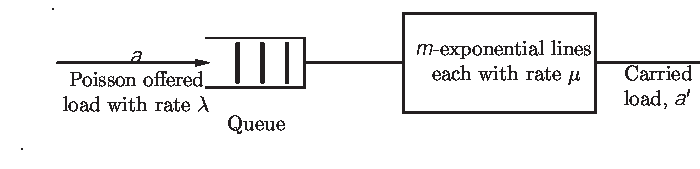
\includegraphics{diagrams/erlangDelayDiagram.eps}\end{center}


\caption{Queueing model of the Erlang delay system.}
\end{figure}
{\small \par}

The Erlang loss system may be analysed as a birth-death process with
birth rate \[
\lambda_{k}=\lambda\]
 and death rate \[
\mu_{k}=\left\{ \begin{array}{cc}
k\mu & k=0,1,\dots,m-1\\
m\mu & k>m\end{array}\right.\]


{\tiny }%
\begin{figure}[ht]
\begin{center}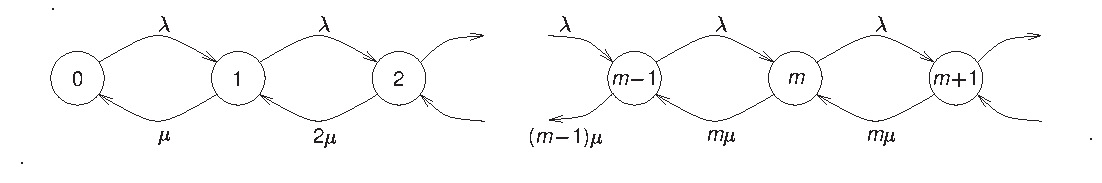
\includegraphics{diagrams/erlangDelay.eps}\end{center}


\caption{State diagram of an Erlang delay system.}
\end{figure}
{\tiny \par}


\rotatefoilhead[-0.5in]{Detailed Balance Equations}

For a system having state less than $m$, $k\leq m$ the detailed
balance equation is 

\[
\lambda P\left(k-1\right)=k\mu P\left(k\right)\]
therefore for $k=0\dots m$ we may write\[
P\left(k\right)=\frac{\lambda}{k\mu}P\left(k-1\right)\]
we define\[
\rho=\frac{\lambda}{m\mu}\]
and therefore\[
\frac{\lambda}{k\mu}=\frac{m\rho}{k}\]
therefore we may write\[
P\left(k\right)=\frac{m\rho}{k}P\left(k-1\right)\]
and as before\begin{eqnarray}
P\left(k\right)=\frac{\left(m\rho\right)^{k}}{k!}P\left(0\right) &  & \textrm{for }k\leq m\label{eq:probabilities}\end{eqnarray}


For systems with state greater than $m$, $k>m$ the detailed balance
equation is\[
\lambda P(k-1)=m\mu P\left(k\right)\]
therefore for $k=m+1\dots\infty$ we may write\[
P\left(k\right)=\frac{\lambda}{m\mu}P\left(k-1\right)\]
and therefore\[
P\left(k\right)=\rho P\left(k-1\right)\]
leading to \[
P\left(k\right)=\rho^{k-m}P\left(m\right)\]
and substituting $k$ with $m$ in (\ref{eq:probabilities}) we can
obtain\[
P\left(m\right)=\frac{\left(m\rho\right)^{m}}{m!}P\left(0\right)\]
therefore \begin{eqnarray*}
P\left(k\right)=\frac{m^{m}\rho^{k}}{m!}P\left(0\right) &  & \textrm{for }k>m\end{eqnarray*}
thus we can write\[
P\left(k\right)=\left\{ \begin{array}{cc}
P\left(0\right)\frac{(m\rho)^{k}}{k!}, & k\leq m\\
P\left(0\right)\frac{m^{m}\rho^{k}}{m!} & k>m\end{array}\right.\]


Once again we can compute $P\left(0\right)$ through normalisation\begin{eqnarray*}
\sum_{k=0}^{\infty}P\left(k\right) & = & 1\\
P\left(0\right)\left[\sum_{k=0}^{m-1}\frac{\left(m\rho\right)^{k}}{k!}+\sum_{k=m}^{\infty}\frac{m^{m}\rho^{k}}{m!}\right] & = & 1\\
P\left(0\right) & = & \left[\sum_{k=0}^{m-1}\frac{\left(m\rho\right)^{k}}{k!}+\sum_{k=m}^{\infty}\frac{m^{m}\rho^{k}}{m!}\right]^{-1}\end{eqnarray*}


consider the second term inside the bracket\[
\sum_{k=m}^{\infty}\frac{m^{m}}{m!}\rho^{k}=\frac{m^{m}\rho^{m}}{m!}\sum_{k=m}^{\infty}\rho^{k-m}\]


substitute in $k^{\prime}=k-m$ and we obtain\[
\frac{m^{m}\rho^{m}}{m!}\sum_{k^{\prime}=0}^{\infty}\rho^{k^{\prime}}=\frac{m^{m}\rho^{m}}{m!}\frac{1}{1-\rho}\]


if $\rho<1$. Thus we have\[
P\left(0\right)=\left[\sum_{k=0}^{m-1}\frac{\left(m\rho\right)^{k}}{k!}+\frac{m^{m}\rho^{m}}{m!\left(1-\rho\right)}\right]^{-1}\]
one quantity of interest is the probability of queueing, $P_{Q}$.
What is the probability, when the system is at steady state, that
a customer will arrive and find all the $m$ servers busy? \[
P\left(k\geq m\right)=\sum_{k=m}^{\infty}P\left(k\right)=P\left(0\right)\sum_{k=m}^{\infty}\frac{m^{m}\rho^{k}}{m!}=P\left(0\right)\frac{\left(\rho m\right)^{m}}{m!}\sum_{k=m}^{\infty}\rho^{k-m}\doteq C\left(m,a\right)\]


making the same substitution as above this can be re-written\[
C\left(m,a\right)=P\left(0\right)\frac{\left(\rho m\right)^{m}}{m!\left(1-\rho\right)}\]


This is known as the \emph{Erlang C formula}, or Erlang's second formula
after A.K. Erlang a pioneer of queueing theory. By defining, $a$,
the offered load to be\[
a=\frac{\lambda}{\mu}=m\rho\]
 and substituting into the above we have \[
C(m,a)=\frac{P\left(0\right)a^{m}}{m!\left(1-\frac{a}{m}\right)}.\]
Nowadays we can compute the probability of waiting on a computer,
however for the purposes of exams and exercises we will use the old
fashioned method of curves.\newcommand{\figureTextSize}{\tiny}

{\small }%
\begin{figure}[ht]
\begin{center}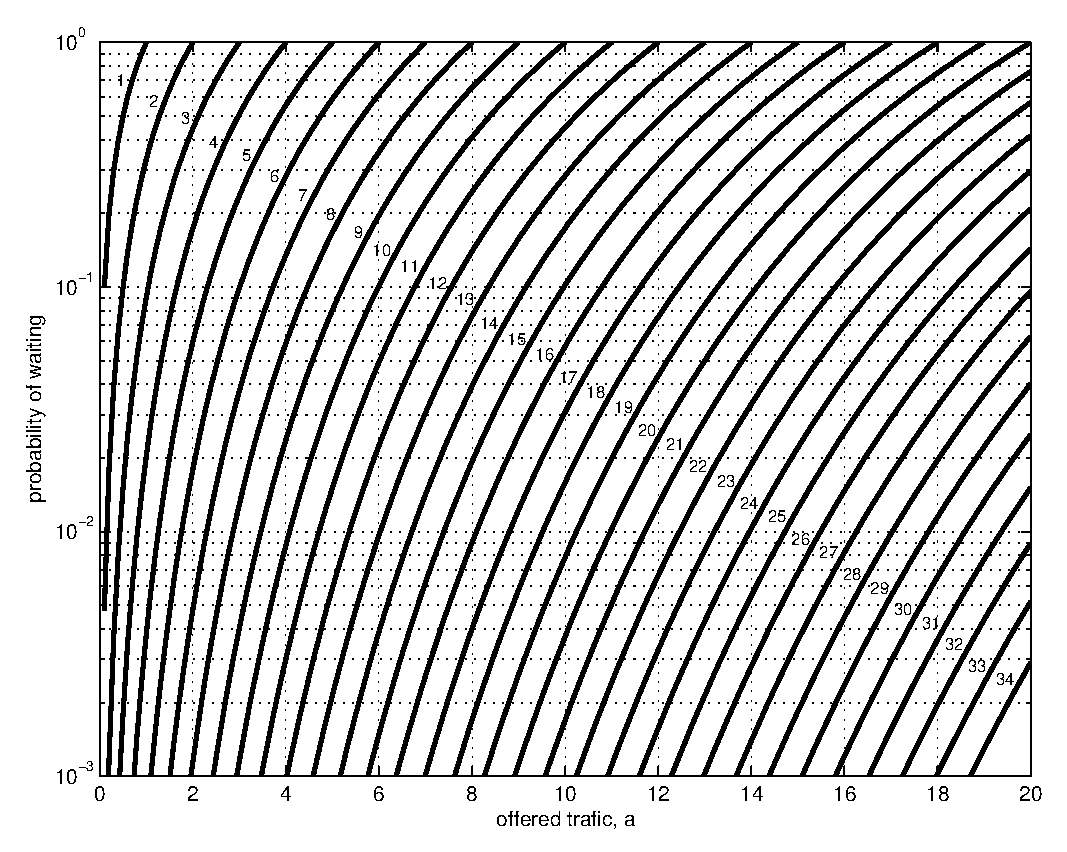
\includegraphics{diagrams/erlangCCurves0to20.eps}\end{center}


\caption{Erlang C curves.}
\end{figure}
{\small \par}

{\small }%
\begin{figure}[ht]
\begin{center}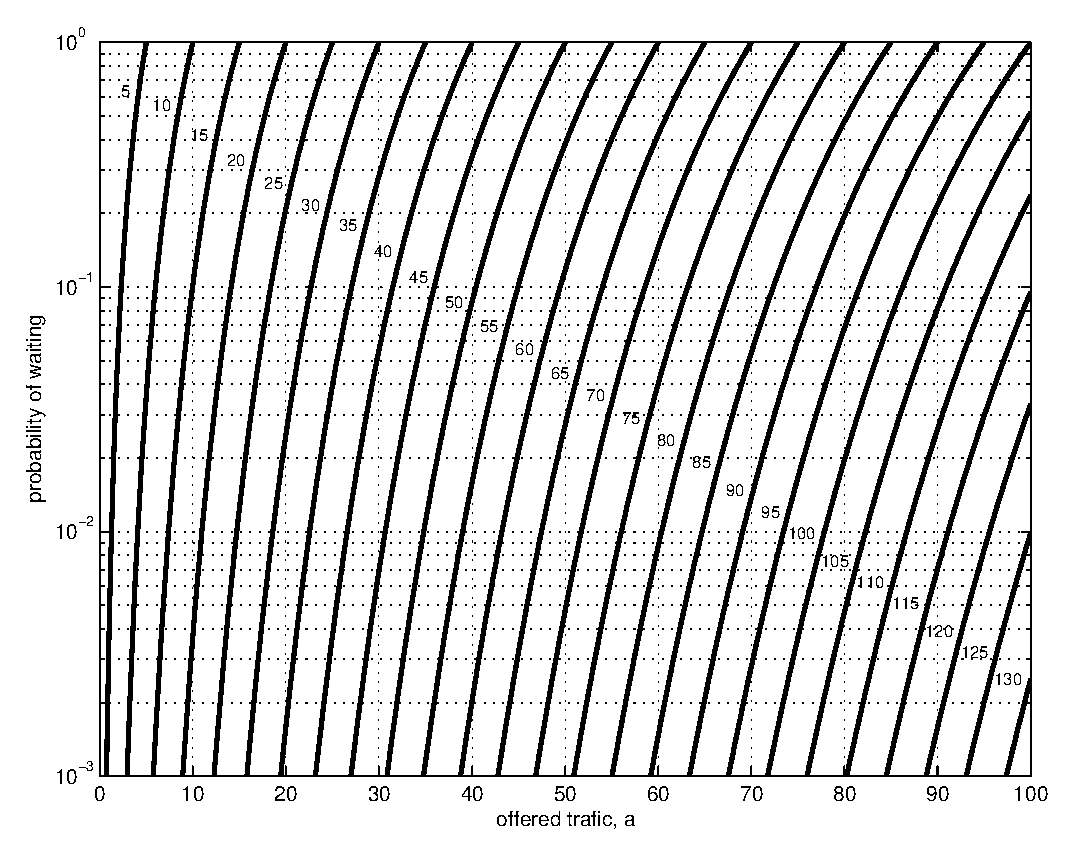
\includegraphics{diagrams/erlangCCurves0to100.eps}\end{center}


\caption{Erlang C curves.}
\end{figure}
{\small \par}


\rotatefoilhead[-0.5in]{$M/M/m$ contd, $M/M/m/m$ and $M/G/1$}

Consider the telephone trunking problem. A telephone exchange A is
to server 10,000 subscribers in a nearby exchange as shown in Figure
\ref{fig:exchange}. Suppose that during the busy hour, the subscribers
generate a Poisson traffic with a rate of 10 calls per minute, which
requires trunk lines to exchange B for an average holding time of
3 minutes per call. Determine the number of trunk lines needed for
a grade of service (probability of waiting) of 0.01.

Average call rate is $\lambda=10$ calls/minute. Average holding time
is $\tau=3$ minutes. Offered load $a=\lambda\tau$ is 30 Erlangs.

From the Erlang C curves it looks to be about 44.

%
\begin{figure}[ht]
\begin{center}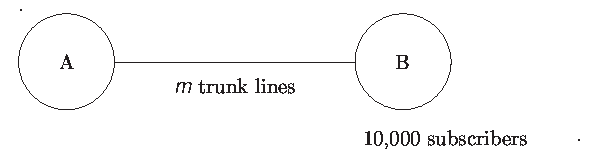
\includegraphics{diagrams/exchange.eps}\end{center}


\caption{The telephone exchange.\label{fig:exchange}}
\end{figure}


A customer service centre has an average holding time, $\tau$, for
calls of 8 minutes. In the busy hour, calls arrive at the centre at
a rate of one very two minutes. Inter-arrival times and service times
are exponentially distributed, how many personel are required to keep
the probability of waiting at 0.1.

From the plot 8.


\rotatefoilhead[-0.5in]{Average number in System.}

The average number of calls in the Erlang Delay System

\[
\bar{N}=\frac{\rho}{1-\rho}C(m,a)+m\rho\]
 These terms represent the average queue length and the average number
of busy lines. \[
\bar{N}_{Q}=\frac{\rho}{1-\rho}C(m,a)\]
 So the average waiting time is simply \[
\bar{W}=\frac{\bar{N}_{Q}}{\lambda}=\frac{C(m,a)}{m\mu(1-\rho)}\]


So what is the average waiting time for the telephone service centre
example? 

$m=8$, $\mu=\frac{1}{8}$, $\rho=\frac{\lambda}{m\mu}=\frac{1}{2}$. 

delay is $\frac{0.1}{8\frac{1}{8}(1-\frac{1}{2})}=0.2$ minutes, or
12 seconds. 


\rotatefoilhead[-0.5in]{Erlang Loss $M$/$M$/$m$/$m$}

%
\begin{figure}[ht]
\begin{center}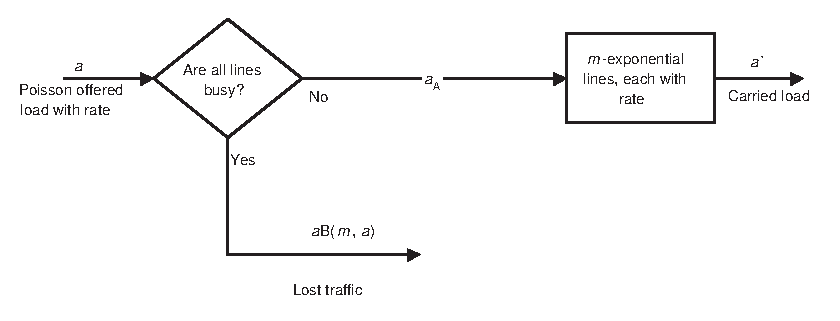
\includegraphics[%
  scale=0.7]{diagrams/erlangLossFlowChart.eps}\end{center}


\caption{Flow chart of the Erlang Loss System.}
\end{figure}


The Erlang loss system may be analysed as a birth-death process with
birth rate \[
\lambda_{k}=\left\{ \begin{array}{cc}
\lambda & k=0,1,\dots,m-1\\
0 & k\geq m\end{array}\right.\]
 and death rate \[
\mu_{k}=\left\{ \begin{array}{cc}
k\mu & k=0,1,\dots,m\\
0 & k>m\end{array}\right.\]
 {[}\emph{Note: for the lower line, it doesn't matter what $\mu_{k}$
is.}{]} 

{\tiny }%
\begin{figure}[ht]
\begin{center}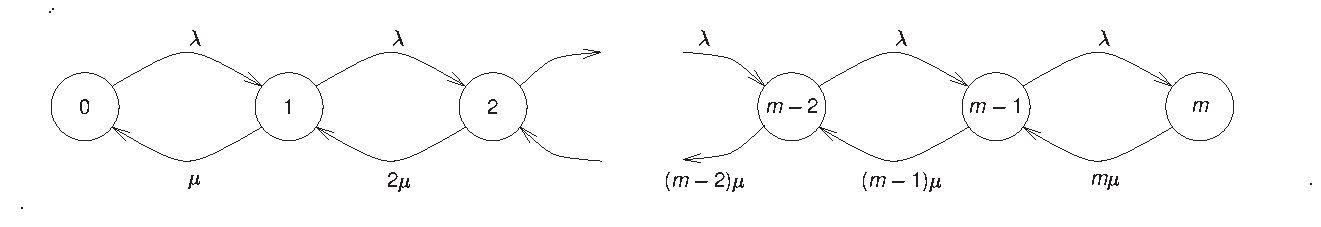
\includegraphics[%
  scale=0.7]{./diagrams/erlangLoss.eps}\end{center}


\caption{Markov chain for the Erlang loss system, $M$/$M$/$m$/$m$}
\end{figure}
{\tiny \par}

The offered load, $a=\frac{\lambda}{\mu}$, is again dimensionless
with units of Erlangs. 


\rotatefoilhead[-0.5in]{Steady State Probabilities}

Using the detailed balance equations we find \begin{eqnarray*}
P\left(k\right) & = & \frac{\lambda_{k}}{\mu_{k}}P(k-1)\\
 & = & \frac{\lambda}{k\mu}P(k-1)\\
 & = & \frac{a}{k}P(k-1)\end{eqnarray*}
 Which means that \begin{eqnarray*}
P\left(k\right) & = & \prod_{n=1}^{k}\frac{a}{n}P\left(0\right)\\
 & = & \frac{a^{k}}{k!}P\left(0\right)\end{eqnarray*}
 The normalisation condition gives us \[
P\left(0\right)\sum_{k=0}^{m}\frac{a^{k}}{k!}=1\]
\[
P\left(0\right)=\frac{1}{\sum_{k=0}^{m}\frac{a^{k}}{k!}}\]
 which leads to the truncated Poisson distribution \[
P\left(k\right)=\frac{\frac{a^{k}}{k!}}{\sum_{n=0}^{m}\frac{a^{n}}{n!}}\]
 Note if $m\rightarrow\infty$ we recover the $M/M/\infty$ queue
as we would expect.


\rotatefoilhead[-0.5in]{Performance Measures for Erlang B}

For the blocking probability and the Erlang B curves we are interested
in the probability that when we arrive the queue is full \[
B(m,a)=P\left(m\right)=\frac{\frac{a^{m}}{m!}}{\sum_{n=0}^{m}\frac{a^{n}}{n!}}\]
 {\small }%
\begin{figure}[ht]
\begin{center}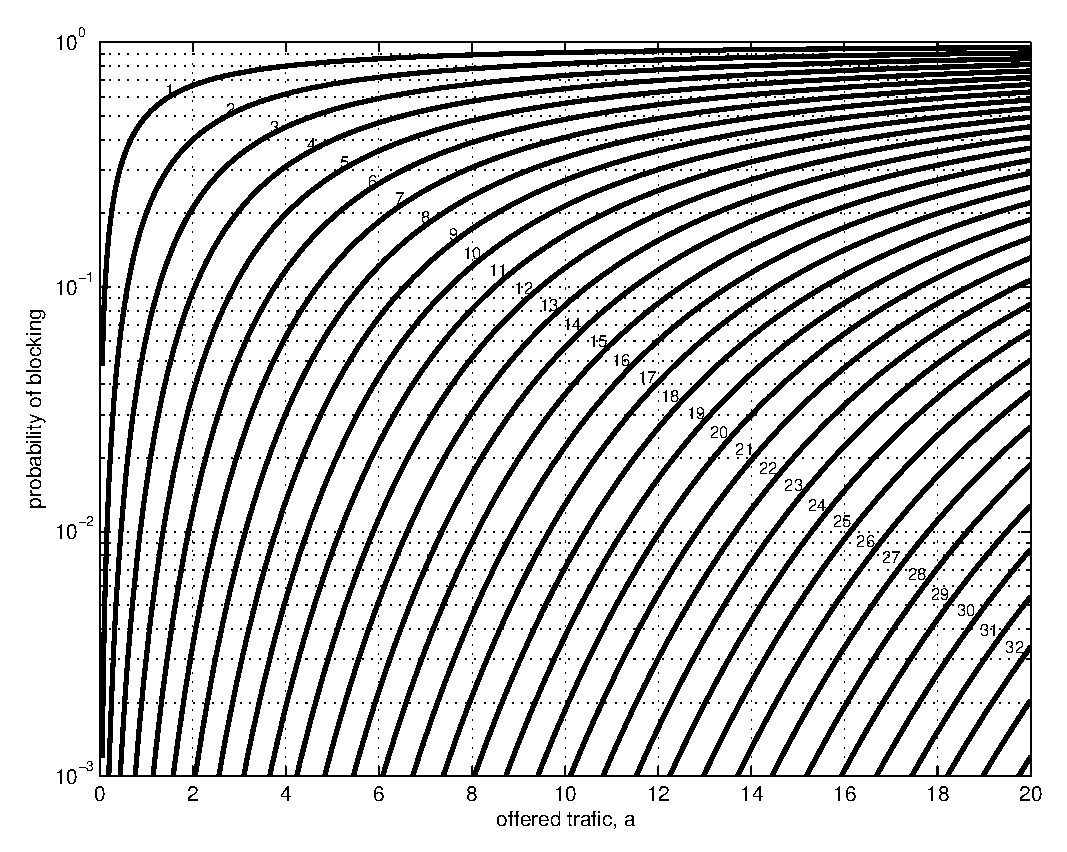
\includegraphics{diagrams/erlangBCurves0to20.eps}\end{center}


\caption{Erlang B curves.}
\end{figure}
{\small \par}

{\small }%
\begin{figure}[ht]
\begin{center}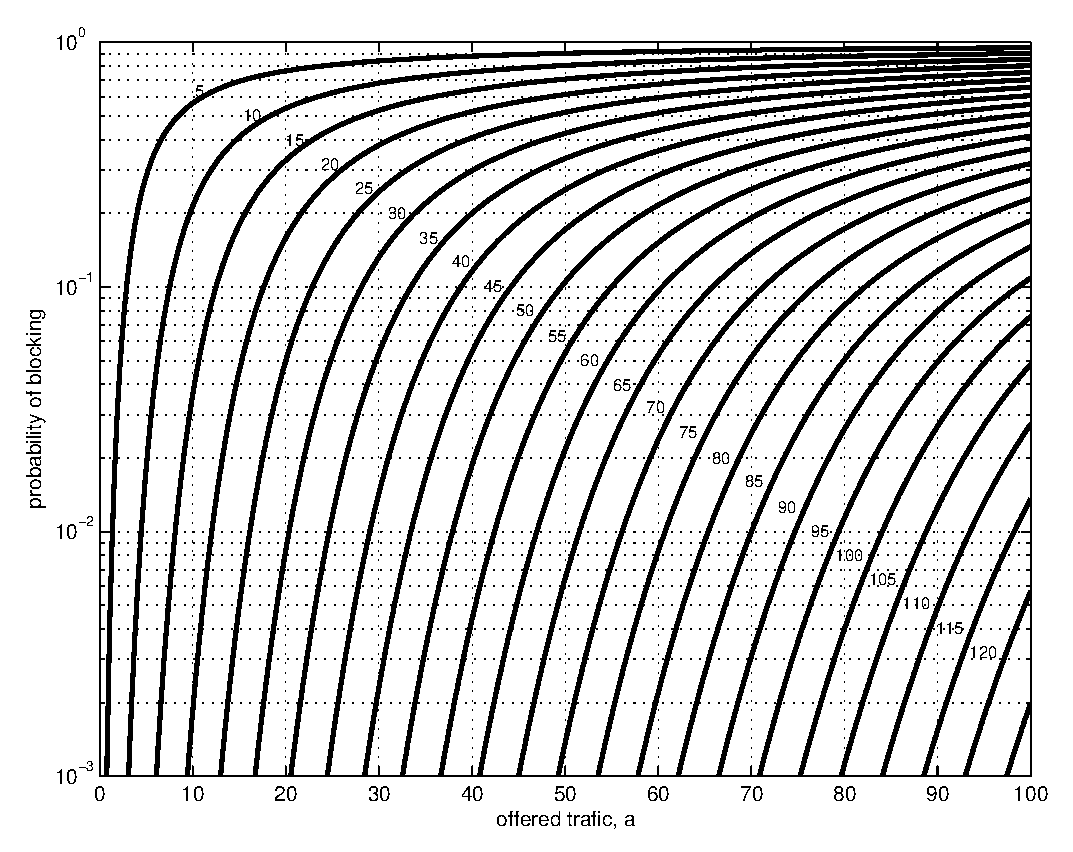
\includegraphics{diagrams/erlangBCurves0to100.eps}\end{center}


\caption{Erlang B curves.}
\end{figure}
{\small \par}


\rotatefoilhead[-0.5in]{Carried Load}

Since traffic is lost in $M/M/m/m$ the carried load, $a^{\prime}$,
is smaller than the offered load. It may be found as \[
a^{\prime}=a(1-P\left(m\right))=a(1-B(m,a))\]
 The carried load per line is the trunk occupancy, \[
\rho=\frac{a^{\prime}}{m},\]
 or the utilization factor --- it is a measure of efficiency of the
line. Note the contrast with the lossless systems where \[
\rho=\frac{a}{m}\]
because $a^{\prime}=a$. 

Load tripling.

For a blocking probability of 0.01, what is the number of trunks needed
for 6 Erlangs of offered load? Answer 12

For a blocking probability of 0.01, what is the number of trunks needed
for 18 Erlangs? Answer 28

So load increase of 200 \% only lead to a trunk increase of 133 \%.
Why? Let's look at the utilization factors. 

\begin{eqnarray*}
\rho_{1} & = & \frac{6}{12}\left(1-0.01\right)=0.495\\
\rho_{2} & = & \frac{18}{28}\left(1-0.007\right)=0.6384\end{eqnarray*}
 The exact utilisation factors The 30 trunk system is thus more efficient.

This explains why it is cheaper to call the U.S.A. than Italy.

Could do with an extra example here.


\rotatefoilhead[-0.5in]{$M$/$G$/$1$ Queue}


\rotatefoilhead[-0.5in]{Pollaczek-Khinchin formula}

If service times are general we cannot use birth death processes to
analyse the system. 

Instead we derive the Pollaczek-Khinchin formula. This formula gives
an expression for the expected waiting time in the queue for any distribution
of service times. \[
\bar{W}=\frac{\lambda\left\langle X^{2}\right\rangle }{2(1-\rho)}\]
 where $\bar{W}$ is expected waiting time, $\left\langle X^{2}\right\rangle =\left\langle X^{2}\right\rangle _{p(X)}$,
$\rho=\lambda\bar{X}$ and $\bar{X}=\left\langle X\right\rangle _{p(X)}$. 


\rotatefoilhead[-0.5in]{Proof of Pollaczek-Khinchin Formula}

We assume that we have a FIFO queue, \emph{i.e.} customers are served
in the order they arrive. We also assume that arrival times are independent
of service times. We will utilise a new concept known as Mean Residual
Service Time. 


\rotatefoilhead[-0.5in]{The Residual Service Time}

Some definitions: 

\begin{tabular}{rcl}
 $W_{i}$&
=&
 Waiting time in queue of $i$th customer.\tabularnewline
 $R_{i}$&
=&
 `Residual service time' seen by the $i$th customer.\tabularnewline
 $X_{i}$&
=&
 Service time of the $i$th customer.\tabularnewline
 $k_{i}$&
=&
 Number of customers in the system when the $i$th customer arrives. \tabularnewline
\end{tabular}

%
\begin{figure}[ht]
\begin{center}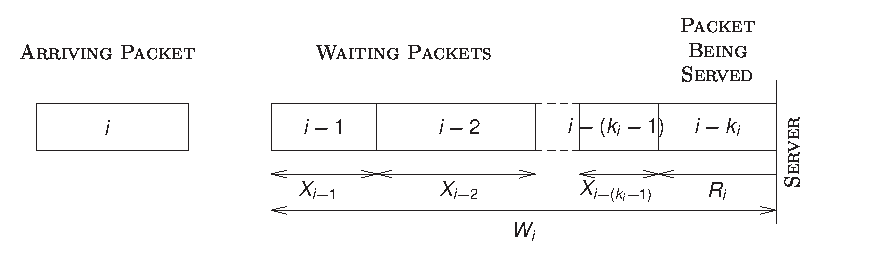
\includegraphics{diagrams/residualServiceOverview.eps}\end{center}


\caption{Graphical representation of residual service time.}
\end{figure}


From these definitions we may immediately write down \[
W_{i}=R_{i}+\sum_{j=i-(k_{i}-1)}^{i-1}X_{j}\]
 summing both sides across $i$ we obtain \[
\sum_{i=1}^{I}W_{i}=\sum_{i=1}^{I}R_{i}+\sum_{i=1}^{I}\sum_{j=i-(k_{i}-1)}^{i-1}X_{j}\]
 dividing through by $I$ gives us \[
\sum_{i=1}^{I}\frac{W_{i}}{I}=\sum_{i=1}^{I}\frac{R_{i}}{I}+\sum_{i=1}^{I}\sum_{j=i-(k_{i}-1)}^{i-1}\frac{X_{j}}{I}\]
 in the limit as $I\rightarrow\infty$ this becomes \[
\lim_{I\rightarrow\infty}\sum_{i=1}^{I}\frac{W_{i}}{I}=\lim_{I\rightarrow\infty}\sum_{i=1}^{I}\frac{R_{i}}{I}+\lim_{I\rightarrow\infty}\sum_{i=1}^{I}\frac{(k_{i}-1)X_{i}}{I}\]
assuming time averages are equivalent to steady state averages this
gives \[
\left\langle W\right\rangle =\left\langle R\right\rangle +\left\langle \left(k-1\right)X\right\rangle \]
 Now since the length of the queue as seen by the $i$th arrival is
independent of the $i$th arrival's length this means $\left\langle (k-1)X\right\rangle =\left\langle k-1\right\rangle \left\langle X\right\rangle $
and since $(k-1)$ is the length of the queue we may write \[
\bar{W}=\bar{R}+\bar{N}_{Q}\bar{X}\]
 Using Little's theorem \[
\bar{N}_{Q}=\lambda\bar{W}\]
 we can obtain \[
\bar{W}=\bar{R}+\lambda\bar{X}\bar{W}\]
 and the fact that $\rho=\lambda\bar{X}$ gives us \[
\bar{W}=\bar{R}+\rho\bar{W}\]
 Leading to \begin{equation}
\bar{W}=\frac{\bar{R}}{1-\rho}\label{eqn:arrivals}\end{equation}
 It remains to calculate $\bar{R}$. 


\rotatefoilhead[-0.5in]{Residual Service Time from Departures Perspective}

Plot of the residual service time over time. Here $M\left(t\right)$
is the number of service completions in the interval $[0,\, t]$.

%
\begin{figure}[ht]
\begin{center}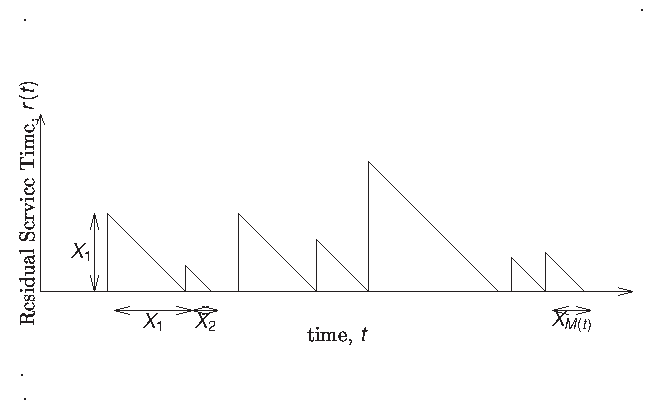
\includegraphics{diagrams/residualTime.eps}\end{center}


\caption{Graphical computation of mean residual time.}
\end{figure}


The time average of the mean residual service time can be calculated
in terms of the area under the curve, $A(t)$ which in turn is the
area under each of the triangles which may be written \[
A(t)=\frac{1}{2}\sum_{i=1}^{M(t)}X_{i}^{2}\]
 The average service time is the area divided by time, $t$. \begin{eqnarray}
\frac{A(t)}{t} & = & \frac{M(t)}{t}\frac{A(t)}{M(t)}\\
 & = & \frac{1}{2}\frac{M(t)}{t}\frac{\sum_{i=1}^{M(t)}X_{i}^{2}}{M(t)}\end{eqnarray}
 As $t\rightarrow\infty$ we find $M(t)\rightarrow\infty$ and \[
\bar{R}=\frac{1}{2}\lambda\left\langle X^{2}\right\rangle .\]
 If we assume that time averages and ensemble averages are equal we
may substitute back into eqn (\ref{eqn:arrivals}) and obtain the
Pollaczek-Khinchin formula \[
\bar{W}=\frac{\lambda\left\langle X^{2}\right\rangle }{2(1-\rho)}\]


This implies that the total waiting time is \[
\bar{T}=\bar{X}+\frac{\lambda\left\langle X^{2}\right\rangle }{2(1-\rho)}\]
 and through Little's formula we can obtain the expected queue length,
$\bar{N}_{Q}$, and the expected number in the system, $\bar{N}$. 

Recall that for an $M$/$M$/$1$ system the service times are exponentially
distributed,

\[
P\left(X\right)=\mu\exp\left(-\mu X\right)\]
this means that\[
\bar{X}=\frac{1}{\mu}\]
 then since the variance of the system is $\frac{1}{\mu^{2}}$\[
\left\langle X\right\rangle ^{2}=\frac{2}{\mu^{2}}\]
Substituting into the Pollaczek-Khinchin formula we obtain \begin{eqnarray*}
\bar{W} & = & \frac{\rho}{\mu\left(1-\rho\right)}\\
 & = & \frac{\rho}{\mu-\lambda}\end{eqnarray*}


Deterministic service times --- each service takes the same amount
of time\[
P\left(X\right)=\delta\left(X-\frac{1}{\mu}\right)\]
where $\delta\left(\cdot\right)$is the Dirac delta function. For
this system \[
\left\langle X\right\rangle =\frac{1}{\mu}\]
and \[
\left\langle X^{2}\right\rangle =\frac{1}{\mu^{2}}\]
\emph{i.e.} the variance is zero as we would expect. Substituting
into the Pollaczek-Khinchin formula we obtain\[
\bar{W}=\frac{\rho}{2\mu\left(1-\rho\right)}\]


In fact we may derive the full range of results for these distributions. 

\begin{center}\begin{tabular}{c|c|c|c}
 Expected value &
 General &
 Exponential &
Deterministic\tabularnewline
\hline
$\bar{W}$&
 $\frac{\lambda}{2(1-\rho)}\left\langle X^{2}\right\rangle $&
 $\frac{\rho}{\mu(1-\rho)}$&
 $\frac{\rho}{2\mu(1-\rho)}$\tabularnewline
 $\bar{T}=\bar{W}+\frac{1}{\mu}$&
 $\frac{\lambda}{2(1-\rho)}\left\langle X^{2}\right\rangle +\frac{1}{\mu}$&
 $\frac{1}{\mu(1-\rho)}$&
 $\frac{2-\rho}{2\mu(1-\rho)}$\tabularnewline
 $\bar{N_{Q}}=\lambda\bar{W}$&
 $\frac{\lambda^{2}}{2(1-\rho)}\left\langle X^{2}\right\rangle $&
$\frac{\rho^{2}}{(1-\rho)}$&
 $\frac{\rho^{2}}{2(1-\rho)}$\tabularnewline
 $\bar{N}=\lambda\bar{W}+\rho=\lambda\bar{T}$&
 $\frac{\lambda^{2}}{2(1-\rho)}\left\langle X^{2}\right\rangle +\rho$&
 $\frac{\rho}{1-\rho}$&
 $\frac{\rho(2-\rho)}{2(1-\rho)}$\tabularnewline
\end{tabular}\end{center}

Uniform Service times --- A uniform probability distribution is defined
between 0 and $b$ for $X>0$ as\[
U\left(X|b\right)=\left\{ \begin{array}{cc}
\frac{1}{b} & 0<X\leq b\\
0 & X>b\end{array}\right.\]
show that the man of this uniform distribution is given by $\frac{b}{2}$
and its variance by $\frac{b^{2}}{12}$ and find the expected waiting
time for an $M/U/1$ queue?

For the mean we have\begin{eqnarray*}
\left\langle X\right\rangle  & = & \int_{0}^{\infty}Xp\left(X\right)dX\\
 & = & \int_{0}^{\infty}XU\left(X|b\right)dX\\
 & = & \int_{0}^{b}\frac{X}{b}dX\\
 & = & \left[\frac{X^{2}}{2b}\right]_{0}^{b}\\
 & = & \frac{b^{2}}{2b}-0\\
 & = & \frac{b}{2}\end{eqnarray*}
For the variance we also require \begin{eqnarray*}
\left\langle X^{2}\right\rangle  & = & \int_{0}^{\infty}X^{2}p\left(X\right)dX\\
 & = & \int_{0}^{b}\frac{X^{2}}{b}dX\\
 & = & \left[\frac{X^{3}}{3b}\right]_{0}^{b}\\
 & = & \frac{b^{3}}{3b}-0\\
 & = & \frac{b^{2}}{3}\end{eqnarray*}
The variance is $\left\langle X^{2}\right\rangle -\left\langle X\right\rangle ^{2}=\frac{b^{2}}{3}-\left(\frac{b}{2}\right)=\frac{b^{2}}{12}$.

\begin{description}
\item [Waiting~Time~For~Queue]For simplicity we consider $\mu=\frac{1}{\left\langle X\right\rangle }.$
So $\mu=\frac{2}{b}$ and thus $b=\frac{2}{\mu}$. So we can write
the second moment in terms of $\mu$. $\left\langle X^{2}\right\rangle =\frac{b^{2}}{3}$,
substituting in $b=\frac{2}{\mu}$ we have $\left\langle X^{2}\right\rangle =\frac{4}{3\mu^{2}}$.
Substituting in to the P-K formula we recover\[
\bar{W}=\frac{2\rho}{3\mu\left(1-\rho\right)}.\]

\end{description}
~

Automatic Repeat Request system --- ARQ System. 

%
\begin{figure}[ht]
\begin{center}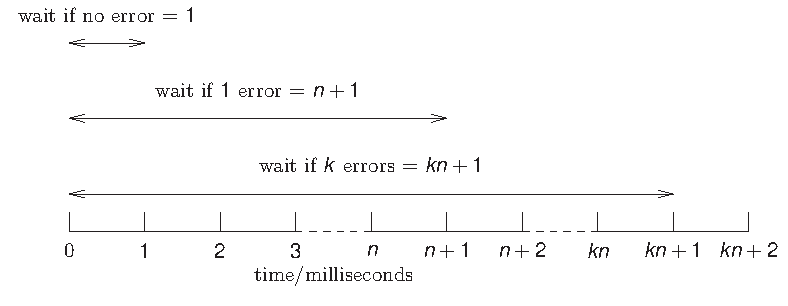
\includegraphics{diagrams/ARQ.eps}\end{center}


\caption{The ARQ System.}
\end{figure}
Assume each packet takes 1 millisecond to be transmitted.

The system waits $n-1$ milliseconds for an acknowledgement. If there
is no acknowledgement the system retransmits.

The probability of an error in a packet is taken to be $p$. Errors
are taken to be independent. Assume that packets arrive as a Poisson
process with rate $\lambda$.  Time interval between transmission
and re-transmission is $1+kn$ time units with probability $\left(1-p\right)p^{k}$

The probability of the service time is\[
P\left(X=1+kn\right)=\left(1-p\right)p^{k}\]
 The expected service time is therefore\begin{eqnarray*}
\left\langle X\right\rangle  & = & \sum_{k=0}^{\infty}\left(1+kn\right)\left(1-p\right)p^{k}\\
 & = & \left(1-p\right)\left(\sum_{k=0}^{\infty}p^{k}+n\sum_{k=0}^{\infty}kp^{k}\right)\\
 & = & 1+\frac{np}{1-p}\end{eqnarray*}
 since $\sum_{k=0}^{\infty}p^{k}=\frac{1}{1-p}$ and $\sum_{k=0}^{\infty}kp^{k}=\frac{p}{\left(1-p\right)^{2}}$.
Thus we can write that\[
\rho=\frac{\lambda\left(1-p\right)}{1-p+np}\]
and thus \[
1-\rho=\frac{1-\lambda-p\left(n-1-\lambda\right)}{1-p+np}\]
The second moment of the service time is\begin{eqnarray*}
\left\langle X^{2}\right\rangle  & = & \sum_{k=0}^{\infty}\left(1+kn\right)^{2}\left(1-p\right)p^{k}\\
 & = & \left(1-p\right)\left(\sum_{k=0}^{\infty}p^{k}+2n\sum_{k=0}^{\infty}kp^{k}+n^{2}\sum_{k=0}^{\infty}k^{2}p^{k}\right)\\
 & = & 1+\frac{2np}{1-p}+\frac{n^{2}\left(p+p^{2}\right)}{\left(1-p\right)^{2}}\end{eqnarray*}
since \[
\sum_{k=0}^{\infty}k^{2}p^{k}=\frac{p+p^{2}}{\left(1-p\right)^{3}}\]
 Substitiuting into the P-K formula gives a very ugly formula!


\rotatefoilhead[-0.5in]{Lectures 15 \& 16}


\rotatefoilhead[-0.5in]{$M/G/1$ Queues with Vacations }

Consider a server which, when it is free, attends to some other business,
for example it could transmit control and record keeping traffic. 

These periods are sometimes known as vacations --- American for holidays. 

\begin{itemize}
\item If a new arrival arrives during a vacation it must wait until the
vacation is over before being dealt with.
\item If a vacation ends and the server is idle it immediately goes on a
new vacation. 
\end{itemize}
~

%
\begin{figure}[ht]
\begin{center}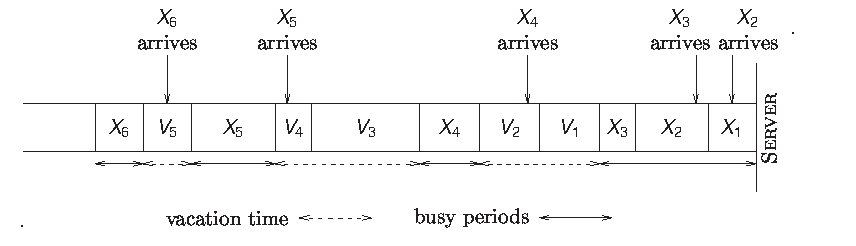
\includegraphics{diagrams/vacationMG1.eps}\end{center}


\caption{Schematic of $M/G/1$ queue}
\end{figure}


We denote the length of these successive vacations to be $V_{1}$,
$V_{2}$, $\dots$. 

We assume that $V_{1},$$V_{2}$, $\dots$ are i.i.d. random variables
which are also independent of the customer times and the service times. 

For a Poisson arrival system with general service times we will look
to compute the average waiting time for a system of this type. 

%
\begin{figure}[ht]
\begin{center}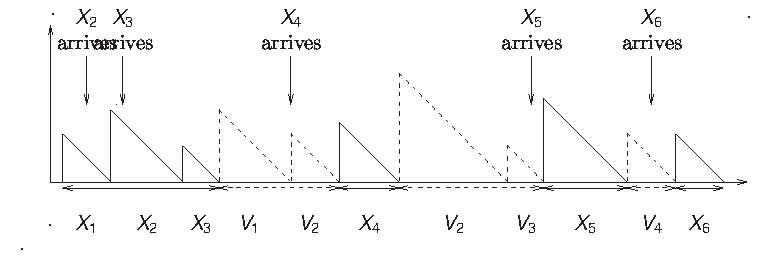
\includegraphics{diagrams/vacationResidual.eps}\end{center}


\caption{Computation of residual service time for system with vacations.}
\end{figure}


For this system \begin{eqnarray}
\frac{1}{t}\int_{0}^{t}r\left(\tau\right)d\tau & = & \frac{1}{t}\sum_{i=1}^{M\left(t\right)}\frac{1}{2}X_{i}^{2}+\frac{1}{t}\sum_{i=1}^{L\left(t\right)}\frac{1}{2}V_{i}^{2}\nonumber \\
 & = & \frac{M\left(t\right)}{t}\frac{1}{2}\frac{\sum_{i=1}^{M\left(t\right)}X_{i}^{2}}{M\left(t\right)}+\frac{L\left(t\right)}{t}\frac{1}{2}\frac{\sum_{i=1}^{L\left(t\right)}V_{i}^{2}}{L\left(t\right)}\label{eq:vacationResidual}\end{eqnarray}


On average the proportion of time available for utilisations is $\left(1-\rho\right)$.
If the average length of a vacation at time $t$ is $\bar{V}_{t}$
then the number of vacations that will have arrived is $L\left(t\right)=\frac{t\left(1-\rho\right)}{\bar{V}_{t}}$.
Therefore if we take the limit of (\ref{eq:vacationResidual}) as
$t\rightarrow\infty$ we find \[
\bar{R}=\frac{1}{2}\lambda\left\langle X^{2}\right\rangle +\frac{\left(1-\rho\right)\left\langle V^{2}\right\rangle }{2\bar{V}}\]


So given that the assumptions that we used to develop the formula 

\[
\bar{W}=\frac{\bar{R}}{1-\rho}\]
are still valid, we may write\[
\bar{W}=\frac{\lambda\left\langle X^{2}\right\rangle }{2\left(1-\rho\right)}+\frac{\left\langle V^{2}\right\rangle }{2\bar{V}}\]


A bar has Poisson arrivals and one member of staff serving. When there
are no customers at the bar, the staff member leaves the bar to check
on the kitchen. Assuming these checks are exponentially distributed
in length, with mean $\bar{V}$ and that customer service times are
exponentially distributed with mean $\bar{X}$ what is the average
waiting time int he queue?

Exponential standard deviation = $\frac{1}{\mu}$, mean$=\frac{1}{\mu}$.
So if mean is $\bar{V}$, standard deviation is $\bar{V}$ and variance
is $\bar{V}^{2}$. Thus second moment is $\left\langle V^{2}\right\rangle =2\bar{V}^{2}$.
Similarly for second moment of service time $\left\langle X^{2}\right\rangle =2\bar{X}^{2}$.
Defining $\rho=\lambda\bar{X}$ we have \[
\bar{W}=\frac{\lambda\bar{X}}{\left(1-\rho\right)}+\bar{V}=\frac{\rho}{\left(1-\rho\right)}+\bar{V}.\]
Determinisitic vacations would have lead to \[
\bar{W}=\frac{\lambda\bar{X}}{\left(1-\rho\right)}+\frac{\bar{V}}{2}=\frac{\rho}{\left(1-\rho\right)}+\frac{\bar{V}}{2}.\]
 


\rotatefoilhead[-0.5in]{Putting Queues Together}

Consider the simple system ivolving two transmission lines in tandem.
Packet lengths are exponentially distributed, arrivals occur as a
Poisson process.

The first queue may be modeled as $M/M/1$. However the second queue
cannot be. This is because a large packet will typically experience
less delay at the second queue than a small one. 

This is a result of the second queue having a chance to clear while
the large packet is under transmission.

In Kleinrock's independence Approximation we simply assume that this
correlation does not exist.

Consider a general network with labelled nodes and links between these
nodes.

There are several packet streams in the network, each stream has a
rate of $x_{s}$. We define $f_{ij}\left(s\right)$ as the fraction
of packets from stream $s$ that cross the link between $i$ and $j$.
The rate associated with a link between node $i$ and $j$ is then
\begin{eqnarray*}
\lambda_{ij} & = & \sum_{s\textrm{ }}f_{ij}\left(s\right)x_{s}.\end{eqnarray*}
Kleinrock suggested that merging traffic streams on a transmission
line has the effect of restoring independence of arrival and service
times. The approach is to assume that each link can be treated as
an $M/M/1$ queue. 

Good approximation for 

\begin{enumerate}
\item arrivals which occur as a Possion process 
\item exponentially distributed packets
\item densely connected networks 
\item moderate-heavy traffic.
\end{enumerate}
Given this assumption, from the $M/M/1$ queue we know that the average
number at each link is \[
\bar{N}_{ij}=\frac{\lambda_{ij}}{\mu_{ij}+\lambda_{ij}}\]
thus the average number in the entire system is\begin{eqnarray*}
\bar{N} & = & \sum_{ij}\bar{N}_{ij}\\
 & = & \sum_{ij}\frac{\lambda_{ij}}{\mu_{ij}+\lambda_{ij}}\end{eqnarray*}
average delay at each link is given by Little's theorem\[
\bar{T}_{ij}=\frac{1}{\mu_{ij}+\lambda_{ij}}\]
%
\begin{figure}[ht]
\begin{center}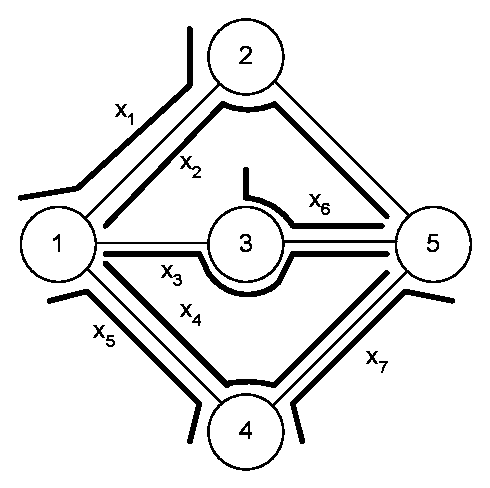
\includegraphics[%
  scale=0.5]{diagrams/kleinrockNetwork.eps}\end{center}


\caption{A small network with five nodes.}
\end{figure}


Figure shows a five node network. Below the rates associated with
the different routes and the average transmission times different
lines are shown. 

\begin{tabular}{cc}
$x_{1}$&
5\tabularnewline
$x_{2}$&
10\tabularnewline
$x_{3}$&
7\tabularnewline
$x_{4}$&
12\tabularnewline
$x_{5}$&
4\tabularnewline
$x_{6}$&
8\tabularnewline
$x_{7}$&
4\tabularnewline
\end{tabular}\begin{tabular}{c|ccccc}
$\mu$&
1&
2&
3&
4&
5\tabularnewline
\hline
1&
-&
-&
-&
-&
-\tabularnewline
2&
20&
-&
-&
-&
-\tabularnewline
3&
20&
-&
-&
-&
-\tabularnewline
4&
30&
-&
-&
-&
-\tabularnewline
5&
-&
20&
20&
30&
-\tabularnewline
\end{tabular}

According to the Kleinrock independence assumption, what is the most
congested link?

From the diagram we can see which links traffic flows down. Let us
take each link in turn

\begin{tabular}{c|ccccc}
$\lambda$&
1&
2&
3&
4&
5\tabularnewline
\hline
1&
-&
-&
-&
-&
-\tabularnewline
2&
$x_{1}+x_{2}=15$&
-&
-&
-&
-\tabularnewline
3&
$x_{3}=7$&
-&
-&
-&
-\tabularnewline
4&
$x_{4}+x_{5}=16$&
-&
-&
-&
-\tabularnewline
5&
-&
$x_{2}=10$&
$x_{3}+x_{6}=15$&
$x_{4}+x_{7}=16$&
-\tabularnewline
\end{tabular}

\begin{tabular}{c|ccccc}
N&
1&
2&
3&
4&
5\tabularnewline
\hline
1&
-&
-&
-&
-&
-\tabularnewline
2&
$\frac{15}{20-15}=3$&
-&
-&
-&
-\tabularnewline
3&
$\frac{7}{20-7}=\frac{7}{13}$&
-&
-&
-&
-\tabularnewline
4&
$\frac{16}{30-16}=1\frac{1}{7}$&
-&
-&
-&
-\tabularnewline
5&
-&
$\frac{10}{20-10}$=1&
$\frac{15}{20-15}$=3&
$\frac{16}{30-16}=1\frac{1}{7}$&
-\tabularnewline
\end{tabular}

The most congested links are from 1 to 2 and 3 to 5.

What is the quickest route between node 1 \& 5?

Need average delay at each link:

\begin{tabular}{c|ccccc}
N&
1&
2&
3&
4&
5\tabularnewline
\hline
1&
-&
-&
-&
-&
-\tabularnewline
2&
$\frac{1}{20-15}=\frac{1}{5}$&
-&
-&
-&
-\tabularnewline
3&
$\frac{1}{20-7}=\frac{1}{13}$&
-&
-&
-&
-\tabularnewline
4&
$\frac{1}{30-16}=\frac{1}{14}$&
-&
-&
-&
-\tabularnewline
5&
-&
$\frac{1}{20-10}=\frac{1}{10}$&
$\frac{1}{20-15}=\frac{1}{5}$&
$\frac{1}{30-16}=\frac{1}{14}$&
-\tabularnewline
\end{tabular}

This means that to go via node 2 takes $\frac{1}{5}+\frac{1}{10}=0.3$
via node 3 takes $\frac{1}{13}+\frac{1}{5}=0.277$ via node 4 it takes
$\frac{1}{14}+\frac{1}{14}=\frac{1}{7}=0.1429$ according to Kleinrock's
independence assumption.

Here we have assumed that there is no further delay associated with
each link (propoagation, processing). In practice such delays may
arise however we shall not consider them. See Bertsekas \& Gallager
Section 3.6.1 for more details.

\bibliographystyle{abbrv}
\bibliography{lawrence,other,zbooks}

\end{document}
